\documentclass[12pt,a4paper,openright,oneside]{article}
\usepackage{amsfonts, amsmath, amssymb,latexsym,amsthm, mathrsfs, enumerate}
\usepackage[catalan]{babel}
\usepackage{epsfig}

\parskip=5pt
\parindent=15pt
\usepackage[margin=1.2in]{geometry}
\usepackage{graphicx}
\usepackage{listings}
\usepackage[utf8]{inputenc}
\usepackage{fancyvrb}
\setcounter{page}{0}


\numberwithin{equation}{section}
\newtheorem{teo}{Teorema}[subsubsection]
\newtheorem*{teo*}{Teorema}
\newtheorem*{prop*}{Proposició}
\newtheorem*{corol*}{Corol·lari}
\newtheorem{prop}{Proposició}[subsubsection]
\newtheorem{corol}{Corol·lari}[subsubsection]
\newtheorem{lema}{Lema}[subsubsection]
\newtheorem{defi}{Definició}[subsubsection]
\newtheorem{nota}{Notació}

\theoremstyle{definition}
\newtheorem{prob}{Problema}
\newtheorem*{sol}{Solució}
\newtheorem{ex}{Exemple}
\newtheorem{exs}{Exemples}
\newtheorem{obs}{Observació}
\newtheorem{obss}{Observacions}

\def\qed{\hfill $\square$}

\renewcommand{\refname}{Bibliografia}
% --------------------------------------------------
\usepackage{fancyhdr}

\lhead{}
\lfoot{}
\rhead{}
\cfoot{}
\rfoot{\thepage}

\begin{document}

\bibstyle{plain}

\thispagestyle{empty}

\begin{titlepage}
\begin{center}
\begin{figure}[htb]
\begin{center}

\includegraphics[width=6cm]{ub.png}
\end{center}
\end{figure}

\textbf{\LARGE Treball final de grau} \\
\vspace*{.5cm}
\textbf{\LARGE GRAU EN ENGINYERIA INFORMÀTICA } \\
\vspace*{.5cm}
\textbf{\LARGE Facultat de Matemàtiques \\ Universitat de Barcelona} \\
\vspace*{1.5cm}
\rule{16cm}{0.1mm}\\
\begin{Huge}
\textbf{EINES BASADES EN TEXT PER A LA VISUALITZACIÓ I GEOLOCALITZACIÓ DE NOTÍCIES} \\
\end{Huge}
\rule{16cm}{0.1mm}\\

\vspace{1cm}


\begin{center}
\textbf{\LARGE Aleix Solanes Font}
\end{center}
\begin{flushright}
\vspace*{2cm}

\renewcommand{\arraystretch}{1.5}
\begin{tabular}{ll}
\textbf{\Large Director:} & \textbf{\Large Dr. Jordi Vitrià Marca} \\
\textbf{\Large Realitzat a:} & \textbf{\Large  Departament de Matemàtica     } \\
 & \textbf{\Large Aplicada i Anàlisi} \\
\\
\textbf{\Large Barcelona,} & \textbf{\Large \today }
\end{tabular}

\end{flushright}

\end{center}










\end{titlepage}


\newpage
\pagenumbering{roman} 

\section*{Abstract} 
This project came up after a few meetings with the professor Dr. Jordi Vitrià talking about Data Science, the possibilities inside this sector, about interesting projects that people made using Data Science, we talked about some cases that could be interesting to analyse, all with a spot in mind, the possibility of reaching a result and visualize that result in an understandable way. So, after those inspiring meetings we achieved the main idea of this project: Geolocation of news. \\ \\
Regarding the journalism sector, hundreds of news are published every day, but unfortunately not all of them include a proper geographic reference. All those news with a reference to a geographic location let the door open to a new way of distribution, and also let new ways of analysis based on this new parameter, the location. \\
As an example, imagine that a developer wants to let a user with a smartphone or a tablet, receive automatically the news related to the place where the user is. Without a reference to where the news took place it is difficult to face the problem, however with a reference to a place the problem now seems affordable.\\ \\
During the realization of this project, various tools and methods are used in order to obtain automatically a set of georeferenced tags from the news and thus be able to show the results in an easy way to analyse. \\
Despite being this project based in the concept of Data Science, I am not explicitly  using algorithms from the world of Data Science (in this report I will explain the reasons why some algorithms could not be used), I follow, however, the main principles: look for databases that can help me face the problem, clean all data in order to be able to use it, and finally I try to show the results in an understandable way to reach results or conclusions. \\ \\
This document outlined in detail the design, development and implementation of every single step that was necessary to achieve the final result.\\ \\
In order to see the results in a simple way, I also created a website with a summary of all the project and some visualizations of the results under the following URL:\\
\begin{center}
\emph{http://alsolanes.github.io/TFG}
\end{center}
\newpage
\section*{Resum}
Aquest projecte va néixer al cap d'algunes reunions amb el professor Dr. Jordi Vitrià en les quals parlàvem sobre Data Science i les seves possibilitats, sobre projectes interessants que la gent havia creat, sobre casos que seria interessant de poder analitzar, i tot amb una fita: la possibilitat d'arribar a algun resultat i fer que aquest es pogués representar visualment d'una forma entenedora. \\\\
En el sector del periodisme es publiquen centenars de notícies cada dia, però malauradament no totes elles inclouen la seva corresponent referència geogràfica. Que una notícia tingui aquesta referència, pot obrir nous camins en la distribució d'aquestes, així com permetre noves opcions d'anàlisi. Per exemple, considerem un desenvolupador que vol permetre a un usuari amb un smartphone o una tablet, que en funció d'on estigui, rebi les notícies automàticament d'aquesta zona. Sense cap referència a aquestes notícies seria difícil encara el problema, no obstant, si disposem d'aquesta informació el problema es simplifica.\\ \\
En el marc d'aquest projecte, s'utilitzaran diferents eines i mètodes per a poder obtenir d'una forma automàtica les referències geogràfiques d'un conjunt de notícies i així poder-ne representar els resultats d'una forma que sigui senzilla d'analitzar posteriorment.\\
Aquest projecte neix de la curiositat que em despertava el món de la Data Science, o més concretament, el poder acabar extraient conclusions d'una sèrie de dades. Si bé no s'utilitzen explícitament algorismes pròpiament del món de Data Science (durant aquesta memòria s'explicaran els motius pels quals alguns algorismes no s'han pogut utilitzar), si que es segueixen les idees fonamentals d'agafar una gran quantitat de dades, netejar-les i finalment mirar de visualitzar les dades per a facilitar la tasca d'obtenció de resultats o conclusions.\\ \\
Per tal de facilitar l'accés als resultats també s'ha habilitat una pàgina web amb el procés resumit així com la visualització dels diferents resultats obtinguts. La direcció en qüestió és:
\begin{quote}
\centering
http://alsolanes.github.io/TFG
\end{quote}

\newpage 


\section*{Agraïments}

\begin{flushright}
\emph{A la meva família que sempre els he tingut al meu costat, donant-me suport en totes les decisions i moments d'aquesta etapa.}
\end{flushright}
\begin{flushright}
\emph{A la Carla, que sense la seva paciència, el seu recolzament en els moments més durs, i la seva complicitat en les alegries, això no hauria estat possible.}
\end{flushright}
\begin{flushright}
\emph{Al Dr. Jordi Vitrià per la passió i la paciència mostrada en cada una de les nostres reunions, tant al parlar del projecte, com en curiositats del món de Data Science.}
\end{flushright}
\newpage

\tableofcontents

\newpage

\pagenumbering{arabic} 
\setcounter{page}{1}
\section{Introducció}
Uns dies abans d'escollir el projecte, vaig tenir l'oportunitat de reunir-me amb el Dr. Jordi Vitrià, per tal de parlar sobre les possibilitats i temes en general relacionats amb Data Science. Durant aquestes converses, van sorgir diferents conceptes, diferents projectes que s'havien realitzat al voltant del món de la Data Science, així com idees que alimentaven la idea de que aprofitant l'oportunitat d'escollir un treball final de grau, seria una bona idea experimentar lleugerament amb algun projecte que hi estigués relacionat.\\
Abans d'introduir el projecte, però, introduiré els conceptes de Big Data i Data Science, ja que en són les arrels.
\subsection{Big Data}
Amb l'evolució de les tecnologies de la informació, s'ha incrementat també la quantitat de dades que es produeixen a internet. En plantejar-se com tractar tota aquesta nova quantitat d'informació, es va veure que per exemple no era viable carregar totes aquestes dades en una base de dades relacional per al seu anàlisis. D'aquesta manera, va aparèixer el concepte de Big Data, per a fer referència a tota aquella informació que no pot ésser processada o analitzada utilitzant processos o eines que hi havia fins aleshores.\\
\subsection*{Quins tipus de dades es poden generar?}
Aquesta gran quantitat d'informació pot venir de diferents fonts, i fins i tot s'ha de tenir en compte que no només aquesta informació és generada pels humans, sinó que existeixen dades creades per màquines, com pot ser el cas de les M2M (Machine-to-Machine).
\begin{figure}[htbp]
\centering
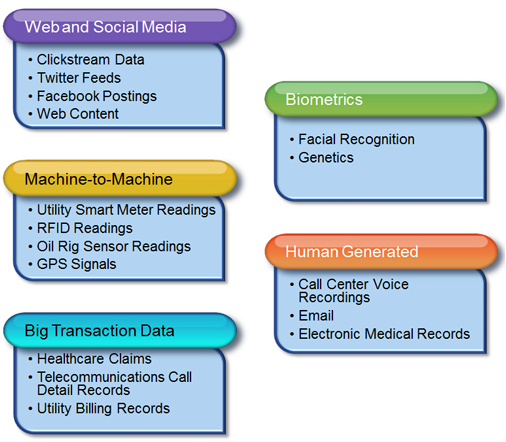
\includegraphics[width=6cm]{tipus_data.png}
\caption{Tipus de dades a analitzar dins el sector Big Data.\cite{datascienceVenn}}
\end{figure}
Tipus de dades:
\begin{itemize}
\item \textbf{Web i xarxes socials}: Es tracta de la informació generada en pàgines web, així com les dades obtingudes a través de les Xarxes Socials.
\item \textbf{Machine-to-Machine(M2M)}: Són les tecnologies que permeten la interconnexió entre dispositius. S'utilitzen dispositius com ara sensors o mesuradors per a generar dades, i fer que un altre màquina pugui interpretar aquestes dades i donar-los-hi sentit.
\item \textbf{Big Transaction Data}: Són dades transaccionals, disponibles tant de forma semiestructurada com no estructurada. Entre els tipus de dades que inclou, s'hi troben per exemple registres de facturació o registres detallats de trucades (CDR).
\item \textbf{Biomètriques}: Són dades biomètriques que inclouen informació sobre empremtes dactilars, escanejos de retina, reconeixement facial, genètica, etc. Són dades especialment importants en els sectors de seguretat. 
\item \textbf{Dades generades per humans}: És la informació que generem al enviar correus, escriure documents electrònics, en fer-nos estudis mèdics, deixar missatges de veu,... 
\end{itemize}
I dins tota aquesta quantitat d'informació hi podríem incloure també la que pot generar una empresa de premsa, la qual genera centenars de notícies a diari amb les seves respectives meta-dades, les imatges, vídeos, i tota la informació que correspongui a cada notícia\cite{BigData}.\\\\
Una vegada tenim totes aquestes dades, és necessari un tractament per a poder mirar d'entendre i extreure'n conclusions, i és aquí on entra el món de la Data Science.
\subsection{Data Science}
Data Science, és un nou camp que està estretament lligat amb l'anàlisi de Big Data, però no es centra exclusivament en projectes de Big Data, ja que l'objectiu principal és l'extracció de coneixement d'una font de dades.

\begin{quote}
\emph{"A Data scientist is somebody who is inquisitive, who can stare at data and spot trends. It's almost like a Renaissance individual who really wants to learn and bring change to an organization."}
\begin{flushright}
- Anjul Bhambhri, vicepresident dels productes Big Data d'IBM.
\end{flushright}
\end{quote}

Les persones que treballen en Data Science, s'anomenen Data Scientists, i la seva formació es basa en tres grans eixos: coneixement del negoci, capacitats en programació, i formació en matemàtiques i estadística.

\begin{figure}[htbp]
\centering
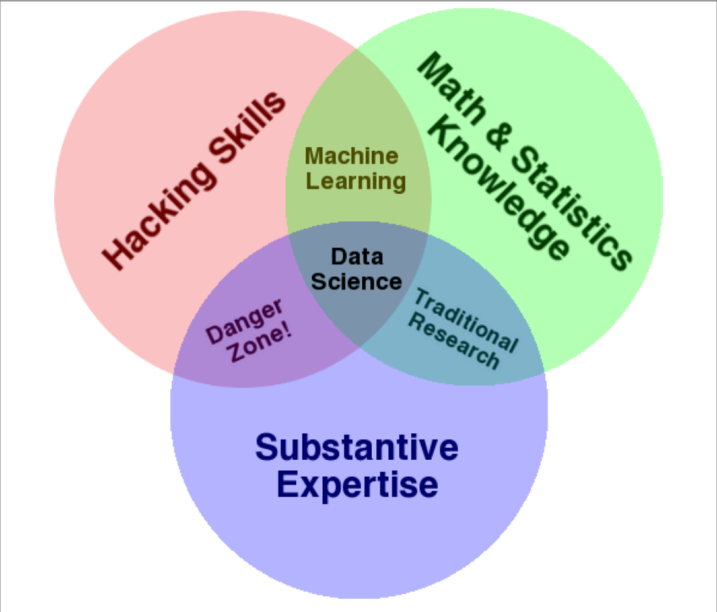
\includegraphics[width=6cm]{conway-datascience.png}
\caption{Diagrama de Venn de Data Science. De Drew Connway.\cite{datascienceVenn}}
\end{figure}
\newpage
Segons Nathan Yau, doctor en estadística per la universitat de UCLA i redactor cap del portal divulgatiu www.flowingdata.com, un expert en Data Science ha de tenir les següents capacitats:
\begin{itemize}
\item Estadística
\item Data munging: capacitat per a manipular i adaptar les dades segons les necessitats (parsing, scraping i formatting data).
\item Visualització de les dades (graphs, mapes,...).
\end{itemize}
L'aparició del terme Data Science, té els seus orígens en els requeriments que demanava per algunes ofertes de feina Google, i que demanaven les següents habilitats per als futurs candidats:
\begin{quote}
\emph{"Persona capaç de treballar amb un equip sobre problemes que requereixen habilitats amb estadística i ciències de la informàtica, juntament amb característiques personals que incloguin la curiositat i la persistència."}
\begin{flushright}
- Exemple de les característiques que empreses com Google solien demanar abans de l'acceptació del terme Data Science, l'any 2008,en els seus futurs candidats.\cite{datasciencejob}
\end{flushright}
\end{quote}
Veient que existia la creixent demanda d'aquest perfil, el Dr. Dhanurjay "DJ" Patil juntament amb Jeff Hammerbacher (Facebook i LinkedIn respectivament) van decidir encunyar el terme "Data Science" per a descriure aquest lloc de treball\cite{datasciencejob} 
\newpage
\subsection{El projecte}

El següent projecte es centra en l'anàlisi d'un conjunt de notícies, i obtenir de cada notícia un o varis punts geogràfics que representaran l'àmbit geogràfic d'on està parlant el text, per a posteriorment mostrar en un mapa els resultats d'aquest anàlisi.\\ \\
Per a poder arribar aquests resultats el procés es divideix en quatre grans etapes:
\begin{enumerate}
\item Recopilació de notícies
\item Cerca i neteja d'una base de dades fiable que contingui noms de localitats i les seves coordenades.
\item Anàlisi del text de cada notícia recopilada per a extreure'n noms de ciutats.
\item Representar les localitats trobades en un mapa.
\end{enumerate}

Totes aquestes etapes s'aniran detallant en el desenvolupament del següent document.\\
Una vegada es tinguin els resultats, els mapes resultants així com una explicació general del procés per arribar-hi, estarà disponible mitjançant una pàgina web pública, des de la qual es posarà el codi a disposició del públic.

\subsection{Antecedents}
A continuació es descriuran una sèrie d'antecedents que guarden una estreta relació amb el projecte. Dels següents casos, no tots tenen les mateixes finalitats i característiques, en concret es poden separar en dos categories: els projectes que pretenen trobar referències geogràfiques en textos, i els que pretenen obtenir les coordenades geogràfiques de diferents punts.\\
El projecte guarda relació amb els diferents projectes donat que es pretén primer geolocalitzar textos i després visualitzar-los en un mapa, i per a fer aquesta visualització es necessita prèviament haver obtingut les coordenades geogràfiques respectives.
\subsection*{Cerca de referències geogràfiques en documents}
\subsubsection*{Yahoo BOSS Geo Services}

\begin{figure}[htbp]
\centering
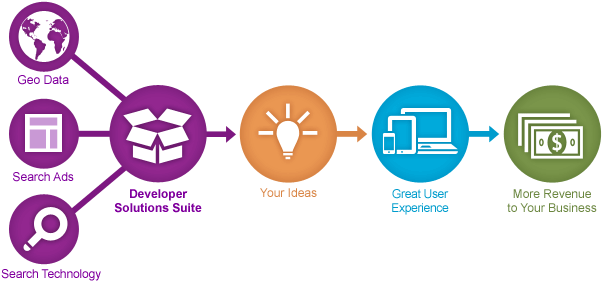
\includegraphics[width=6cm]{Yahoo_boss.png}
\caption{Esquema de negoci de Yahoo BOSS}
\end{figure}
Yahoo BOSS Geo Services, és un servei web que es divideix en dos projectes:
\begin{itemize}
\item PlaceFinder: Permet als seus usuaris trobar les coordenades concretes d'una direcció o localitat.
\item PlaceSpotter: Donat un text que pot pertànyer a un twit de twitter, una notícia, una pàgina web, entre altres, retorna les localitats que ha pogut localitzar dins d'aquest text.
\end{itemize}
És un servei de pagament, i el seu cost varia en funció del nombre de consultes diàries que es desitgin fer.\cite{BOSS}
\subsubsection*{CLAVIN}
\begin{figure}[htbp]
\centering

\includegraphics[width=6cm]{clavin.png}
\caption{Logotip del projecte CLAVIN.}
\end{figure}
CLAVIN (Cartographic Location And Vinicity INdexer) és un projecte open source que té com a objectiu assignar "tags" a un document d'entrada especificant la geolocalització d'aquest text. Per a analitzar el text, combina diferents eines open source per a aplicar un processament de llenguatge natural i finalment, amb l'ajut d'un Gazeteer
\footnote{Diccionari geogràfic que conté correspondències entre informació geoespacial i noms.},
 poder trobar les paraules referents a punts geogràfics correctament. Està especialitzat amb treballar sobre grans quantitats d'informació, Big Data, i és per això que per a processar aquestes grans quantitats de dades utilitza el framework Hadoop\footnote{Framework de software que permet treballar amb milers de nodes i amb petabytes de dades.}.\\\\
Com a exemple de funcionament, aprofitarem que la seva pàgina web permet testejar la seva aplicació (http://clavin.berico.us/clavin-web/). Agafarem un text qualsevol en anglès (en qualsevol altre idioma no funciona).\\
\newpage
\begin{figure}[!htbp]
\centering
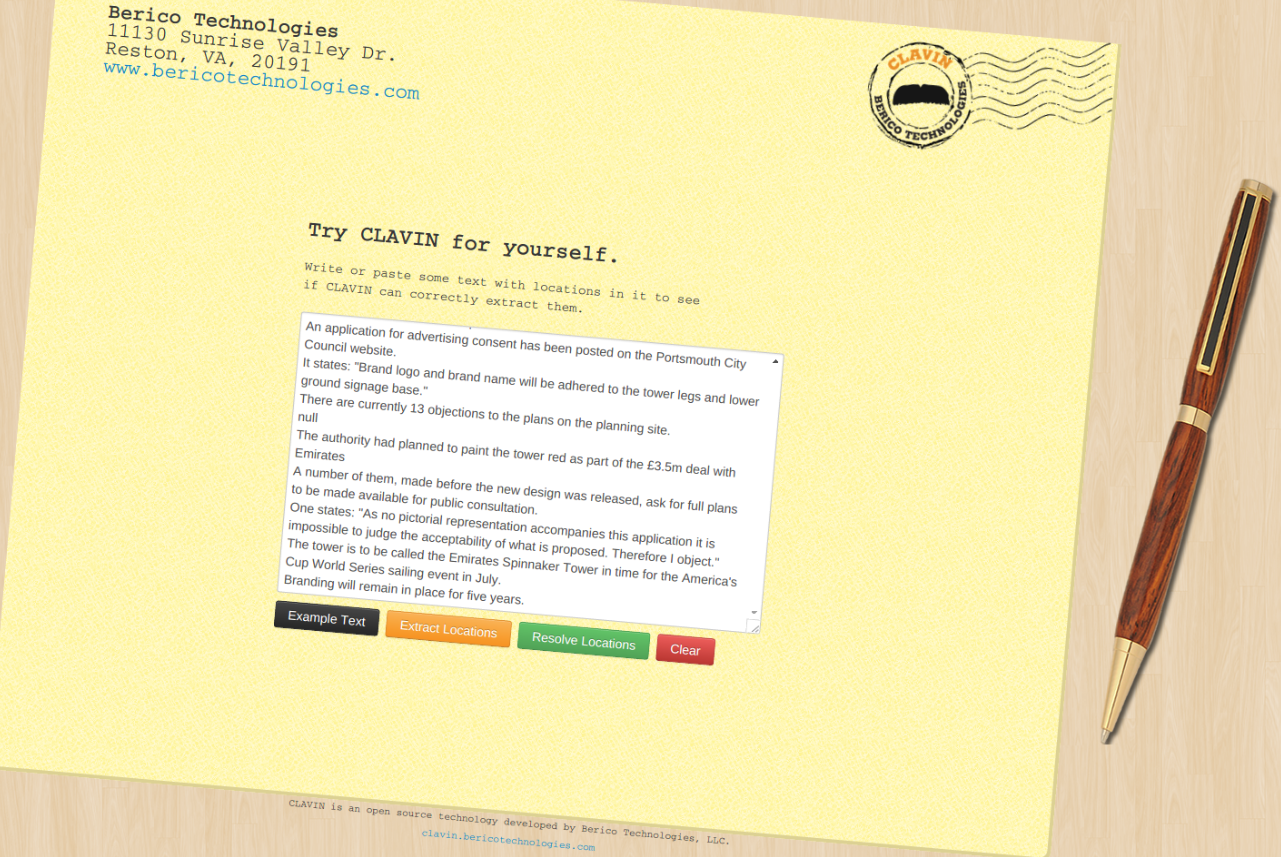
\includegraphics[width=9cm]{clavin-1.png}
\caption{Pàgina web que permet testejar el funcionament del parsejador de punts geogràfics.\cite{clavin}}
\end{figure}
El text parla sobre un edifici de Portsmouth que el volen pintar dels colors de l'equip rival de futbol de la ciutat, i d'on a simple vista es poden localitzar com a ciutats d'on parla la notícia les ciutats de Portsmouth, Hampshire i Southampton.

\begin{figure}[htbp]
\centering
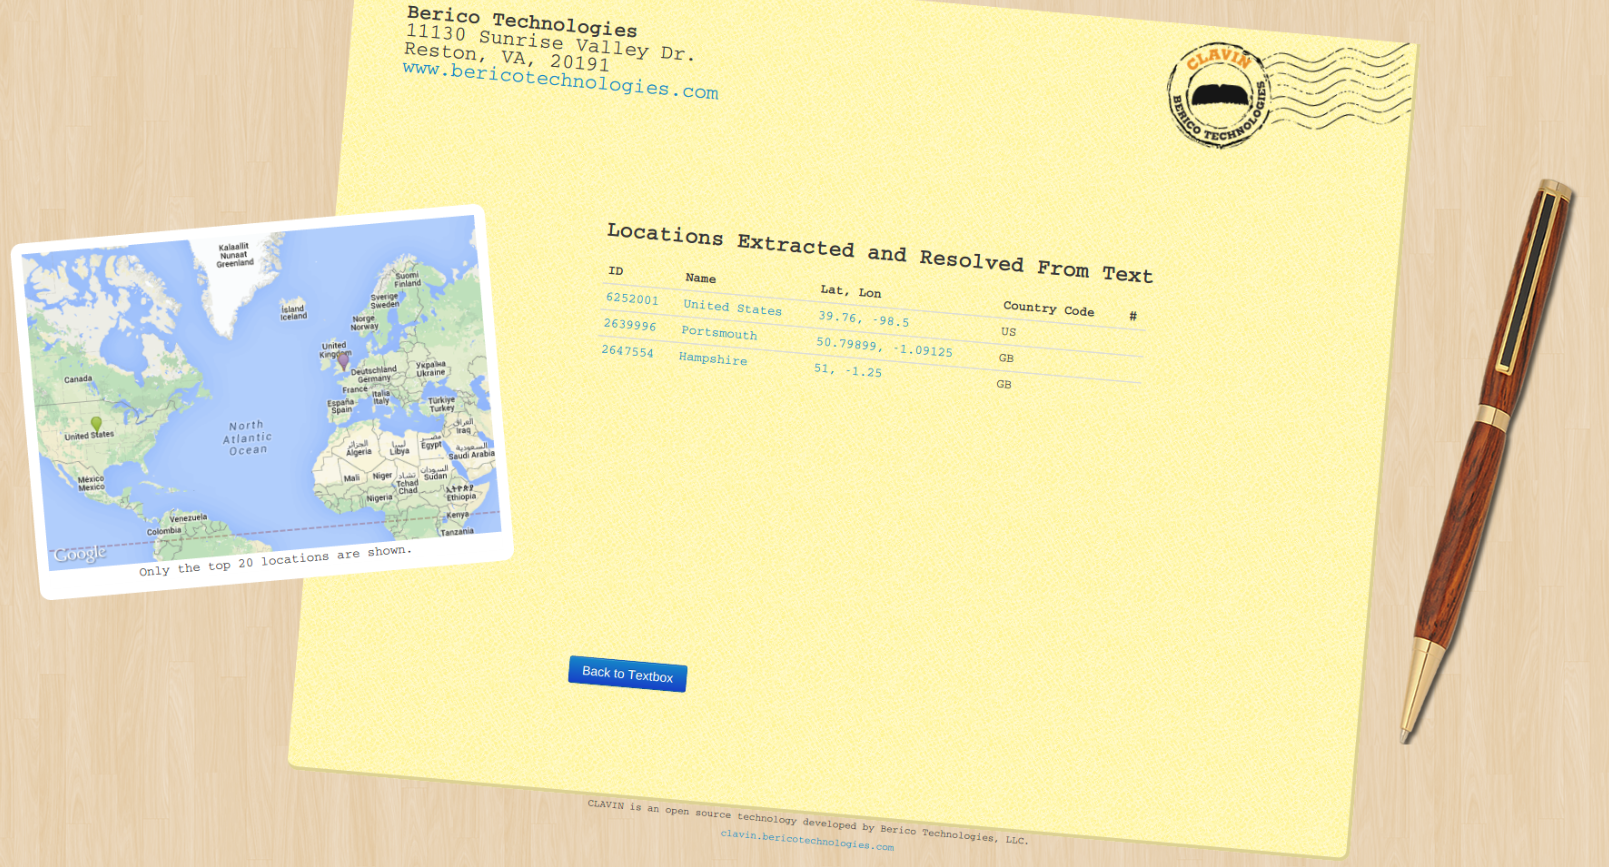
\includegraphics[width=9cm]{clavin-2.png}
\caption{Pàgina web que mostra a la part esquerra un mapa amb les ciutats trobades, i a la dreta la llista de ciutats junt amb les seves coordenades i el país.\cite{clavin}}
\end{figure}Podem comprovar com els resultats que ens indica són les ciutats de Portsmouth i Hampshire, mentre que no ha posat la ciutat de Southampton, donat que la notícia en general no parla de Southampton i només ho menciona pel seu equip de futbol. També posa com a resultat els Estats Units en general.\cite{clavin}
\newpage
\subsubsection*{TextGrounder}
TextGrounder és un projecte que pretén trobar mencions en un text sobre llocs geogràfics o referències temporals. Per a poder retornar la informació correctament, utilitza mètodes de processat de llenguatge natural (NLP) juntament amb algorismes de machine learning per a analitzar el context de la paraula i fer més fiable el resultat donat.\\
Aquest projecte va néixer al setembre de l'any 2010 de les mans de Jason Baldridge (Universitat d'Austin) amb la intenció d'analitzar les referències temporals i geogràfiques en textos acadèmics anglesos del segle XIX.\\
Actualment està compost de tres subprojectes:
\begin{itemize}
\item Geolocalització de documents: Identifica la localització d'un document fent servir bases de dades d'entrenament, les quals contenen distribucions d'unigrames o bigrames que serveixen per a caracteritzar un text. Els textos utilitzats per a entrenar la base de dades principalment són textos de la Wikipedia.
\item Geolocalització de topònims: Identifica cada topònim d'un document i crea un model estadístic per a caracteritzar el text, igual que en l'anterior subprojecte, però en aquest cas s'utilitza un gazeteer\footnote{Diccionari amb referències geogràfiques.} per a verificar aquests topònims.
\item Generador KML: Genera una sèrie de fitxers KML que contindran informació estadística sobre una sèrie de paraules, identificant per exemple les paraules més utilitzades al parlar d'una regió concreta de la terra.\cite{textgrounder}
\end{itemize}
\subsection*{Obtenció de coordenades de punts geogràfics}
\subsubsection*{Google Maps API}
La informació, basada en la base de dades dels seus mapes, està disponible a través d'aquesta API. Google ofereix dues versions de la API, una lliure i la versió "for work". La primera és una versió limitada, que ens permet realitzar un màxim de 2500 consultes per dia i el projecte on s'utilitzi ha de ser gratuït per a tots els públics.\\
La seva utilització es basa en fer crides a un webservice passant-li una sèrie de paràmetres. Així per exemple si desitgem les coordenades d'una direcció concreta, fariem:\\
\begin{figure}[htbp]
\begin{verbatim}
https://maps.googleapis.com/maps/api/geocode/json?
address=585+Gran+Via+de+les+Corts+Catalanes,+Barcelona+,+ES&key=API_KEY
\end{verbatim}
\caption{Crida al webservice de la API de Google}
\end{figure}
\\
Aquesta crida, ens retornaria una resposta JSON la qual contindria informació sobre aquesta direcció, informant-nos del tipus d'edifici que es tracta, la latitud i la longitud.\cite{googleAPI}\\

\subsection{Estructura de la Memòria}
La següent memòria estarà estructurada de forma que primer s'explicaran els \textit{objectius i la definició del problema} per tal de tenir clar quina és la finalitat del treball. \\\\
A continuació es detallaran les diferents etapes de disseny i desenvolupament fins a arribar al resultat final. També es mencionaran aproximacions alternatives a la realització del problema que s'han intentat durant la realització del projecte. Aquesta informació estarà a la secció de \textit{Desenvolupament}.\\\\
A continuació, a la secció \textit{Metodologia i resultats}, es parlarà sobre les metodologies utilitzades durant la realització d'aquest projecte, així com les correspondències entre els resultats esperats, i els resultats reals.\\\\
Finalment, en l'apartat de \textit{Conclusions i vies de continuació}, s'analitzarà el resultat final del treball, i es detallaran les possibles futures ampliacions que es podrien fer al treball, així com possibles solucions per a reduir les limitacions que s'han trobat durant la realització del projecte.

\newpage

\section{Definició d'objectius i motivació del problema}
\subsection{Objectius}
Aquest projecte té com a principal finalitat permetre identificar els punts geogràfics on una notícia té lloc. Però per a poder arribar a aquest punt, s'han d'assolir una sèrie d'objectius on cada un d'ells té un pes igualment important per a poder obtenir uns resultats fiables. Els principals objectius marcats durant el projecte són:
\begin{enumerate}
\item Recopilar una sèrie de notícies per a poder ser analitzades
\item Crear una base de dades fiable amb les localitats que es tindran en compte per a la geolocalització de les notícies.
\item Permetre identificar, donat un text, les paraules que són susceptibles de ser una localitat.
\item Fent servir les bases de dades anteriors, mostrar en un mapa els diferents punts trobats, per a mostrar tant la evolució temporal, com el nombre total d'aparicions d'una localitat en les notícies.
\item Crear una pàgina web per a mostrar-ne els resultats, així com a permetre que altres usuaris puguin continuar o analitzar el desenvolupament.
\end{enumerate}
\subsection{Problema}
En el sector del periodisme, es publiquen centenars de notícies cada dia. Per exemple, la font de referència utilitzada, el diari Ara en la seva versió digital, crea al voltant de 120 notícies diàries.\\
Cada una d'aquestes notícies conté una sèrie de "tags", no obstant, aquestes paraules no sempre segueixen un ordre lògic, o senzillament no permeten categoritzar les notícies segons la seva ubicació geogràfica.
\subsubsection{Cicle de vida d'una notícia}
El cicle de vida d'una notícia conté tres grans etapes:
\begin{itemize}
\item Producció
\item Distribució
\item Consum
\end{itemize}
\newpage
\subsubsection*{Producció d'una notícia}
Durant la producció, és el procés en què el periodista crea la notícia, l'escriu i li assigna una sèrie de paraules que permetran identificar aquesta notícia. Aquestes paraules, poden ser noms de persona que hi apareixen, noms d'empresa, alguna paraula clau,... però no necessàriament ha de contenir la localitat d'on s'està parlant, donat que sovint resta a disposició del periodista assignar les paraules que ell cregui rellevants per al text que ha escrit.\\
\subsubsection*{Distribució d'una notícia}
En aquesta etapa, la notícia ja ha estat creada, revisada, se li han assignat unes paraules clau, s'ha introduït a la base de dades del diari, i ja està en el punt de quedar a la disposició dels clients o usuaris que desitgin accedir a aquesta notícia. La distribució es pot fer en físic o en digital, tot i que en el nostre cas ens centrarem en la part digital. Aquesta distribució es sol realitzar a través de mètodes de distribució com ara RSS (Really Simple Syndication), a través de la seva pàgina web, o d'alguna aplicació mòbil.\\
\subsubsection*{Consum d'una notícia}
Finalment, l'usuari té la notícia a la seva disposició i la pot estar consultant. En aquesta etapa, no hi intervé res més que l'usuari, la notícia en sí i el terminal des d'on l'estigui consumint, ja que qualsevol etapa extra com podria ser el fet que s'ordenin o categoritzin les notícies es consideraria dins l'etapa de distribució d'aquesta.
\\\\
Aquest projecte pretén ser una ajuda per a les etapes de producció (permetent per exemple ajudar a l'escriptor de la notícia a localitzar paraules susceptibles de ser localitats mencionades en la notícia), i per la distribució (permetent tenir les notícies categoritzades segons la zona geogràfica on té lloc la notícia).
\subsection{Exemple del que es pretén aconseguir}
A continuació es mostrarà pas a pas els objectius que es pretenen obtenir fent servir una notícia d'exemple.\\
La notícia que s'analitzarà és una notícia del diari Ara amb el següent text:
\begin{center}
\emph{"Va ser un llunyà juny del 2002 quan el llavors ministre de Medi Ambient, Jaume Matas, i el president de la Generalitat, Jordi Pujol, van col·locar a \textbf{Tiurana} (Noguera) la primera pedra del canal de reg Segarra-Garrigues. Poc podien imaginar tots dos que la seva trajectòria política quedaria enfangada als tribunals, com tampoc podien preveure que el projecte del canal, una de les obres hidràuliques més ambicioses de la història i amb uns primers plànols que es remunten al 1959, tindria 13 anys després el seu futur enlaire."\cite{ara}}
\end{center}
En el text hi podem localitzar la paraula Tiurana, la qual pertany a una petita població de la Noguera. També apareix el nom i cognom de l'expresident de la Generalitat Jordi Pujol. El cognom "Pujol", també correspon a una localitat pertanyent a la comarca del Pallars Sobirà.\\
Una vegada es tinguin les bases de dades corresponents amb les localitats i les seves coordenades, s'espera que el resultat de la geolocalització del text, retorni solament la paraula Tiurana, donat que en aquest cas Pujol és un cognom i no una localitat.\\\\
El resultat de l'etapa de localització de localitats en un text retornaria: \\\emph{Tiurana}. \\ 
Ara el que es voldrà, és trobar-ne les coordenades geogràfiques. Per a dur a terme aquest pas, s'haurà de consultar el nom trobat (\emph{Tiurana}) en la base de dades de localitats. Aquesta consulta s'espera que retorni la informació següent:

\begin{itemize}
\item Nom: Tiurana
\item Latitud: 41.9752700
\item Longitud: 1.2560800
\item Tipus: Poble
\end{itemize}
A aquesta informació se li adjuntarà la font de la notícia, en aquest cas el diari Ara, i la data en què s'ha publicat la notícia, en aquest cas el 2 de maig de 2015. Seguidament es guardarà en una base de dades, junt amb la resta de ciutats trobades en les diferents notícies, i es penjarà el fitxer resultant a la web CartoDB.\\
Una vegada les dades estiguin correctament penjades, es podrà visualitzar cada un dels punts trobats en un mapa. \\
Com que s'inclourà la informació relativa a la data de publicació i també la informació del diari, s'espera que es puguin visualitzar les dades en ordre temporal, i també poder aplicar un filtre per a poder mostrar la informació relativa a un diari en concret.\\\\
L'última etapa consistirà en que tota aquesta informació estigui disponible en una pàgina web junt amb els mapes i una breu descripció del procés per a poder divulgar els resultats del projecte i facilitar a tots els desenvolupadors que ho desitgin accés al codi.
\newpage
\section{Desenvolupament}
Per al procés de desenvolupament del projecte s'han fet servir diferents eines que han facilitat les diferents etapes del procés. Cada tecnologia utilitzada facilita una aproximació al problema, és per això, que també és interessant mencionar altres tecnologies que s'han pogut experimentar durant aquest projecte, tot i que finalment algunes d'elles no s'han utilitzat per al desenvolupament final.\\ 
Tot seguit en presento primer les tecnologies utilitzades, i a continuació altres tecnologies que facilitarien una visió diferent del problema.
\subsection{Eines utilitzades}
\subsection*{Github}
\begin{figure}[htbp]
\centering

\includegraphics[width=7cm]{github.jpg}
\caption{Logotip de Github.}
\end{figure}
És una plataforma de desenvolupament col·laboratiu, que permet allotjar projectes utilitzant un sistema de control de versions GIT. Això permet, que en cas de necessitar-ho, en un moment donat es puguin revertir els canvis, i retornar a una versió anterior.\\
La seva funció més interessant és la de compartir el codi de forma pública, cosa que permetrà que un desenvolupador que vulgui continuar, millorar, o senzillament analitzar el projecte, ho pugui fer a través de la plataforma Github.\\\\
Tot el codi del projecte estarà disponible a GITHUB per a que qualsevol persona el pugui tenir a la seva disposició.\cite{github}
\subsection*{Python}
\begin{figure}[htbp]
\centering

\includegraphics[width=7cm]{python.png}
\caption{Logotip de python.}
\end{figure}
És un llenguatge de programació interpretat, que té com a filosofia principal fer que el codi final resulti llegible i entenedor. \\
És un llenguatge de programació multi-paradigma, és a dir, permet aplicar diferents estils de programació, com ara programació orientada a objectes, programació imperativa o programació funcional.\\
Serà el llenguatge principal per al desenvolupament del projecte.\cite{python}
\newpage
\subsection*{IPython \& Jupyter}
\begin{figure}[htbp]
\centering
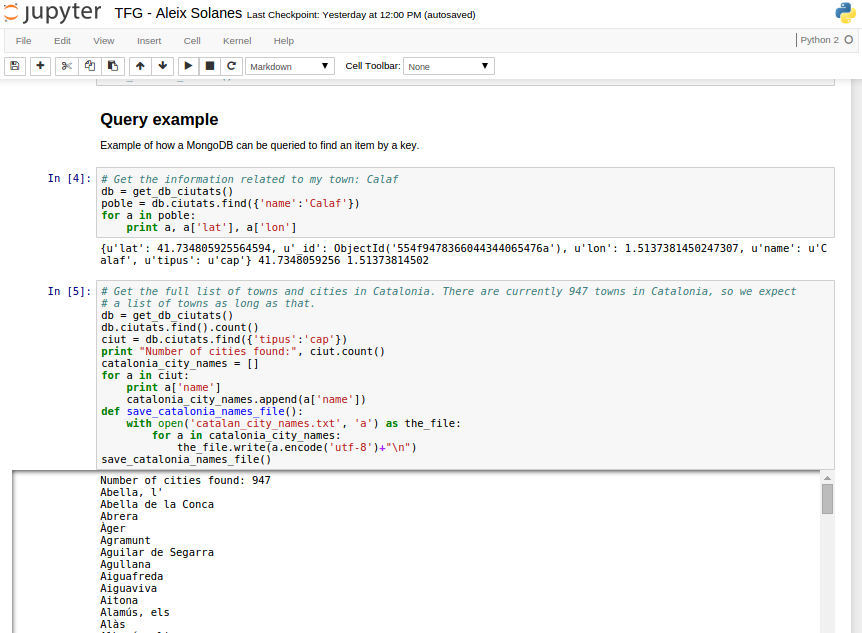
\includegraphics[width=9cm]{ipython.png}
\caption{Exemple d'una notebook Jupiter amb IPython.}
\end{figure}
És un terminal interactiu, que permet funcionalitats extra respecte al terminal per defecte de python, com pot ser per exemple l'autocompletat de variables, mòduls o atributs. Combinat amb el programari \emph{Jupyter}, es permet l'ús de \emph{notebooks} en un navegador. Això permetrà tenir en una mateixa pàgina, fragments de codi amb la seva respectiva execució, i de forma seqüencial poder executar aquests fragments.\\\\
Per a la realització del projecte s'ha optat per la utilització de IPython i Jupyter com a entorn de programació, i Python com a llenguatge.\cite{ipython}
\subsection*{RSS}
RSS és l'acrònim de Really Simple Syndication. Es tracta d'una sèrie de formats de canal web basat en XML. Permeten compartir continguts que s'actualitzen de forma contínua, sovint solen ser notícies, weblogs o podcasts. Aquesta informació sol ser utilitzada per altres programes que en permeten la lectura o visualització.\\\\
Per al projecte, s'utilitzen les fonts de notícies RSS de diferents diaris catalans.\cite{rss}
\subsection*{MongoDB}
El terme MongoDB, ve de l'anglès (humongous database). És un programari de codi obert, per a la creació i gestió de bases de dades orientada a documents. Les seves principals virtuts són la escalabilitat i un alt rendiment.\\
La seva base de dades, emmagatzema la informació sota el format BSON (binary Json).\\\\
En aquest projecte s'utilitzarà per a emmagatzemar les diferents bases de dades de ciutats i de notícies.\cite{mongodb}
\subsection*{JSON}
JSON (Javascript Object Notation) és un estàndard obert basat en text, dissenyat per a l'intercanvi de dades, el qual sigui llegible pels humans.\\
Aquest format es sol utilitzar per a transmetre dades estructurades en una connexió en xarxa.\\\\
Per a emmagatzemar informació que després pugui ésser consultada, utilitzarem el format JSON al guardar alguns fitxers.\cite{json}
\subsection*{CartoDB}
CartoDB és un servei de software web SAAS (software as a service). Permet representar bases de dades amb informació cartogràfica de forma senzilla, permetent a més, personalitzar la visualització per a mostrar diferents tipus de representacions de les dades, com per exemple visualitzar mapes d'evolució temporal, mapes de calor, o de densitat.\\\\
El resultat final del projecte es visualitzarà utilitzant la plataforma CartoDB.\cite{cartodb}
\subsection{Fonts de les dades}
En aquest projecte, s'utilitzaran diverses fonts de dades, i cada una d'elles tindrà les seves particularitats.
\subsection*{RSS - Diaria Ara, Vilaweb, Regió7}
Per a obtenir les dades, es farà servir la descàrrega d'aquestes mitjançant la tecnologia RSS. S'han escollit els diaris Ara, Vilaweb i Regió 7, com a fonts de dades, donat que proveeixen serveis RSS per a poder accedir a les seves notícies.
\subsection*{Geonames}
Per a tenir una relació de ciutats a nivell mundial junt amb les seves coordenades, s'utilitzarà la base de dades disponible a geonames.org. Aquesta base de dades és actualitzada constantment per la comunitat, i en origen, aquestes dades solen provenir de fonts oficials.\cite{geonames}
\subsection*{ICC - Institut Cartogràfic de Catalunya}
L'Institut Cartogràfic de Catalunya, permet des de la seva pàgina web descarregar-se diferents arxius amb informació sobre el territori català. Per a aquest projecte s'utilitzarà la base de dades referent al Nomenclàtor, que conté punts geogràfics de Catalunya, junt amb les seves coordenades i altra informació.\cite{icc}
\subsection*{Github.io}
Per a allotjar el projecte final, i permetre'n la seva divulgació s'utilitzarà la tecnologia facilitada per GITHUB, que de forma senzilla permet crear un enllaç al projecte allotjat a Github. D'aquesta forma qualsevol persona que ho desitgi podrà veure de forma resumida el procés i la implementació final seguida durant aquest projecte.\cite{github.io}
\subsection{Una visió alternativa, altres eines}
En el procés d'investigació de tecnologies i mètodes per a realitzar cada etapa del projecte s'han anat descobrint i provant diferents mètodes. Entre els quals es destaquen els següents:
\subsection*{NLP (Natural Language Processing)}
El procés del llenguatge natural (NLP en anglès), és una disciplina que s'encarrega de tractar computacionalment les llengües naturals, o llengües humanes.\\
Els objectius que ens permetrien una millor identificació de localitats serien:
\begin{itemize}
\item Anàlisi lèxica: Categories gramaticals i sentits de les paraules.
\item Anàlisi morfològica: Gènere, nombre, sufixos... de les paraules.
\item Anàlisi sintàctica: Funcions de cada paraula dins de l'oració, connexió entre oracions, ordre de les paraules...
\item Interpretació semàntica: Forma lògica, independent de l'idioma i del context.
\end{itemize}

Per a Python es disposen de llibreries NLTK(Natural Language ToolKit) que facilitarien la seva implementació en el projecte.\cite{nlp}
\subsubsection*{NER (Named-Entity Recognition}
Dins el processament de llenguatge natural, ens interessaria també especialment, l'apartat de reconeixement d'entitats, el NER (Named-Entity Recognition).\\
Aquesta tasca permetria identificar en un text les diferents entitats, ja siguin noms de persones, de localitats, percentatges, valors monetaris,...\cite{ner}
\subsection*{SPARQL}
En les primeres etapes del projecte, s'ha experimentat amb una tecnologia anomenada SPARQL (SPARQL Protocol and Query RDF Language). Es basa en llenguatge RDF, el qual és un llenguatge per a fer consultes semàntiques en bases de dades.\\Per a demostrar-ne l'ús primer s'ha d'explicar què és la DBPedia, ja que és la font que s'utilitzarà per a l'exemple.\cite{sparql}\\
\subsection*{DBPEDIA}
El llenguatge SPARQL s'ha utilitzat per a intentar obtenir una base de dades utilitzant la base de dades DBPedia. Aquesta base de dades, utilitza com a font principal la wikipedia, i es va actualitzant conforme aquesta rep modificacions.\\
Com a exemple, la següent consulta ens retornarà punts geogràfics de la DBPedia que continguin especificades les coordenades:

\begin{figure}[!htbp]
\begin{verbatim}
PREFIX rdf: <http://www.w3.org/1999/02/22-rdf-syntax-ns#>
PREFIX yago: <http://dbpedia.org/class/yago/>
PREFIX dbpedia-owl: <http://dbpedia.org/ontology/>

SELECT ?title ?geolat ?geolong
WHERE {
    ?place foaf:name ?title .
    ?place geo:lat ?geolat .
    ?place geo:long ?geolong .
}
\end{verbatim}
\caption{Consulta d'exemple amb SPARQL.}
\end{figure}
\newpage
Aquesta consulta ens retornaria la següent taula:

\begin{figure}[htbp]
\centering
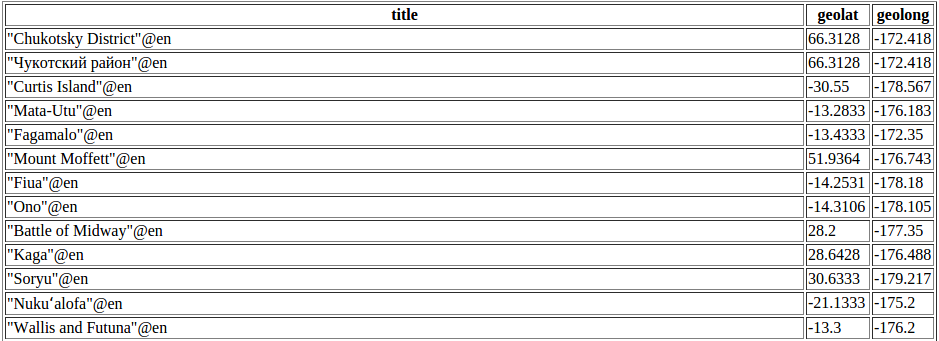
\includegraphics[width=12cm]{sparql-2.png}
\caption{Resultat de la consulta anterior.}
\end{figure}
Aquesta aproximació, tot i ser curiosa i interessant, no proporciona resultats prou fiables com per a ser utilitzada en la implementació final del projecte.\cite{dbpedia}
\subsection{Preparació de l'entorn MongoDB i conceptes bàsics}
Per a la gestió de les bases de dades que s'han utilitzat en el projecte, s'utilitzarà una aproximació NoSQL, MongoDB. Utilitzar una base de dades NoSQL no és una elecció que s'hagi pres sense motiu, ja que es buscava una escalabilitat i una agilitat que una base de dades relacional SQL clàssica no proporcionava.\\
En definitiva el que es necessita és, partint d'un model clau-valor, fer cerques ràpides que retornin un valor al especificar una clau, i en això, els models NoSQL són idonis. Més concretament, MongoDB emmagatzema les seves bases de dades en format BSON (Binary JSON). BSON és una serialització amb codificació binària d'una sèrie de documents amb format JSON. Cada document o objecte, és el que es podria considerar com una espècie d'equivalent del que es coneix com a taula amb termes SQL. \\ \\
Així doncs, una vegada definit l'entorn que s'utilitzarà per a la gestió de les bases de dades, es procedeix a la seva inicialització. La qual en un entorn python ens resultarà especialment simple fent servir la llibreria \emph{PyMongo}. Una vegada s'ha engegat el servidor de la base de dades, que per executar-lo en un entorn Linux s'ha d'executar la comanda "\emph{sudo mongod}", la inicialització bàsica és tan simple que amb dues línies de codi Python permet deixar apunt per a ser utilitzada la nostra base de dades.:

\begin{figure}[!htbp]
\begin{verbatim}
client = MongoClient('localhost:27017')
db = client.ciutats
\end{verbatim}
\caption{Inicialització d'una base de dades MongoDB amb la llibreria PyMongo.}
\end{figure}
Ara que ja es té inicialitzada la base de dades, afegir una ciutat amb les seves corresponents dades, serà fer un \emph{insert} com el següent:

\begin{figure}[!htbp]
\begin{verbatim}
db.ciutats.insert({"name":name, "tipus":tipus,"lat":lat, "lon":lon})
\end{verbatim}
\caption{Insert a una base de dades utilitzant PyMongo.}
\end{figure}
On "\emph{name}" serà el nom del camp, i \emph{name} el seu valor.\\ \\
Per a poder fer consultes sobre una base de dades MongoDB, es pot utilitzar la comanda find de la llibreria PyMongo.

\begin{figure}[htbp]
\begin{verbatim}
db.ciutats.find({'name':'Calaf'})
\end{verbatim}
\caption{Exemple de consulta bàsica utilitzant PyMongo.}
\end{figure}
Com podem veure en la figura anterior, per a fer una consulta bàsica utilitzant l'instrucció \emph{find}, només cal que especifiquem quin camp estem buscant i el valor concret d'aquest. En aquest cas la consulta ens retornaria una estructura JSON amb la informació disponible per al municipi de Calaf com la següent:
\begin{figure}[!htbp]
\begin{verbatim}
{u'lat': 41.734805925564594, u'_id': ObjectId('554f947836604436a'), 
u'lon': 1.5137381450247307, u'name': u'Calaf', u'tipus': u'cap'}
\end{verbatim}
\caption{Exemple de resposta d'una consulta bàsica utilitzant PyMongo.}
\end{figure}
\newpage
\subsection{Obtenció i neteja de les dades}
La primera etapa del procés de desenvolupament del projecte, ha estat la cerca de les bases de dades corresponents, que d'una forma fiable pugui permetre arribar a uns resultats acceptables. És una de les etapes del projecte més importants, donat que qualsevol resultat que se'n desprengui depèn estrictament d'aquestes dades. Per a poder trobar la base de dades final se n'han hagut de provar unes quantes, i fer la corresponent recerca. Fins i tot s'han intentat desenvolupaments alternatius per a construir manualment les bases de dades, com s'explica en la secció de \textit{desenvolupaments alternatius}.\\ \\
En aquesta secció, s'explicarà els processos seguits per tal d'\emph{obtenir}, \emph{analitzar}, i \emph{processar} totes les bases de dades utilitzades en el projecte, per tal de poder-les utilitzar en la següent etapa sense problemes, considerant que hi haurem deixat només la informació important, i en el cas que sigui necessari haurem adaptat el format d'algunes dades per a facilitar la seva utilització.\\ \\
En la introducció, hem parlat sobre el terme Data Science. Si recordem les tres habilitats que el Dr. Nathan Yau mencionava com a pilars en qualsevol Data Scientist (Estadística, Data munging i Visualització de les dades), aquesta etapa faria referència al terme "\emph{Data munging}". Aquest terme, ve del verb en anglès "Munge", el qual significa "transformar dades d'una forma indefinida".
\subsubsection*{D'on extreure les bases de dades?}
En aquest projecte, s'han utilitzat dues aproximacions per a l'obtenció de les bases de dades. Una és senzillament buscar una font fiable i descarregar-la, com en el cas de les ciutats i els seus punts geogràfics; l'altra, donada la impossibilitat de trobar de forma senzilla una base de dades que s'ajustés a les necessitats, ha estat crear-la, buscant un lloc d'on extreure les dades i emmagatzemant-la en una base de dades pròpia, com en el cas de l'obtenció de les notícies a analitzar.
\subsubsection*{Perquè modificar les bases de dades obtingudes?}
S'ha de tenir present, que quan es facilita una base de dades, se'n sol especificar el format per tal que qualsevol persona que la vulgui utilitzar sàpiga com tractar-la. Per desgràcia, cada llenguatge pot tenir les seves particularitats alhora de tractar amb dades, i per això pot ser necessari donar un format concret a les dades prèviament obtingudes. \\També s'ha de tenir en compte, que una base de dades pot incloure molta informació que de bon principi ja se sap que no és necessària per a la implementació d'un projecte, i en aquests casos, per temes d'agilitat i d'espai, també pot ser interessant destriar-ne aquella que resulti innecessària.


\newpage
\subsection*{Base de dades de pobles i ciutats de Catalunya}
Per tal d'obtenir uns resultats el més bons possible, és molt important que les bases de dades que s'utilitzin continguin informació el màxim de fiable. És per això, que després de que s'hagin investigat i provat diferents alternatives, s'ha decidit optar per una base de dades facilitada per l'Institut Cartogràfic de Catalunya, la qual inclou més de 52.000 referències geogràfiques del territori català. Aquesta base de dades està disponible al públic sota el següent enllaç:
\begin{quote}
http://www.icc.cat/index.php/Home-ICC/Publicacions/Nomenclator
\end{quote}
Aquesta informació, que s'ha definit com a base de dades, en un principi és considerat un Nomenclàtor. Aquest terme, fa referència a un document amb informació sobre un nucli poblacional, que pot ésser inferior a una unitat poblacional com pot ser el municipi (nucli de població, llogarets, parròquies,...), i en detalla informació sobre en quina forma s'hi assenta la població. A més, en facilita informació geogràfica, com ara les seves coordenades, cosa que és el que més interessa per a la realització del treball.\\
El primer pas abans de prosseguir és veure quins diferents tipus de dades inclou aquesta base de dades.

\begin{table}[htbp]
\begin{center}
	\centering
    \begin{tabular}{| l | l | l | l |}
    \hline
    \textbf{Abreviació} & \textbf{Significat} \\ \hline
    'cap' & Cap de municipi \\ \hline
	'barri' & Barri, sector urbà (superior a 50.000 habitants)\\ \hline
	'nucli' & Nucli de població(poble, llogaret...)\\ \hline
	'diss.' & Veïnat disseminat \\ \hline
	'e.m.d.' & Entitat municipal descentralitzada \\ \hline
	mun. & Nom del municipi quan aquest no coincideix amb la capital \\ \hline
	edif. & Edificació aïllada\\ \hline
	edif. hist. & Edifici històric (ermita, església, castell,...)\\ \hline
    \end{tabular}
\end{center}
\caption{Tipus de dades inclosos en el nomenclàtor del ICC.\cite{icc}}
\end{table}
Es pot veure doncs, que el que interessa més per aquest projecte és el terme 'cap', que fa referència a Cap de municipi. Per a comprovar que és el que s'entén com a municipi, senzillament es comprova que hi ha 947 referències sota el terme 'cap.', el mateix nombre exacte de municipis que es troben registrats a Catalunya.
\subsubsection*{Estructura de les dades}
El document que inclou tota la informació del nomenclàtor, és un document en format .xlsx (document específic del programa Microsoft Excel, a partir de la seva versió 2007). Per tant, el primer pas en obtenir unes dades, és veure'n el format, per a saber com encarar la seva refactorització per a poder utilitzar-la en el projecte.
\newpage
\begin{figure}[htbp]
\centering
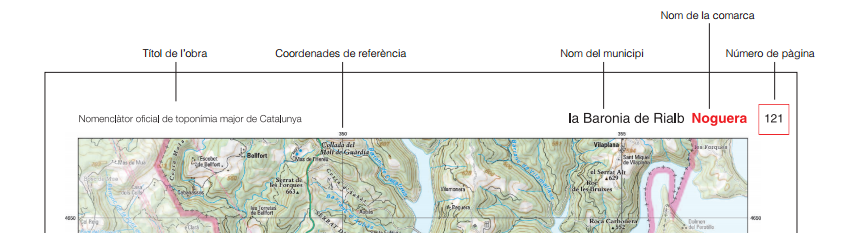
\includegraphics[width=15cm]{nomenclator.png}
\caption{Nomenclàtor oficial de toponímia major de Catalunya.}
\end{figure}
Aquest fitxer d'Excel, fa referència al nomenclàtor oficial de toponímia major de Catalunya, una obra que inclou informació concreta per a cada municipi de Catalunya. És per això que en els termes que analitzarem a continuació hi podem trobar camps de referència a aquesta obra, com ara els camps Volum o el camp pàgina, que indiquen la localització dins la obra física del municipi especificat.\\
Anem a veure les diferents columnes del fitxer d'Excel:
\begin{itemize}
\item \textbf{Topònim}: Nom del punt geogràfic.
\item \textbf{Concepte}: Tipus d'assentament poblacional ('cap', nucli, barri, diss.,...)
\item \textbf{Municipi 1}: Indica el municipi al qual pertany el topònim en qüestió, inclou 4 camps (Municipi 1, Municipi 2, Municipi 3, Municipi 4) a la taula, que indiquen el cas en que pugui pertànyer a múltiples municipis.
\item \textbf{Comarca 1}: Indica a la comarca que pertany el topònim. Pot pertànyer a fins a 5 comarques, per tant inclou 5 camps (Comarca 1, Comarca 2, ..., Comarca 5).
\item \textbf{UTM X i UTM Y}: Coordenades X i Y en el Sistema de Coordenades Universal Transversal de Mercator.
\item \textbf{Volum}: Indicador que fa referència al volum físic de l'obra (Nomenclàtor Oficial de toponímia major de Catalunya).
\item \textbf{Pàgina}: Indicador que fa referència a la pàgina dins el volum físic de l'obra.
\item \textbf{UTMX i UTMY}: Coordenades precises X i Y en el Sistema de Coordenades Universal Transversal de Mercator.
\end{itemize}
\begin{figure}[htbp]
\centering
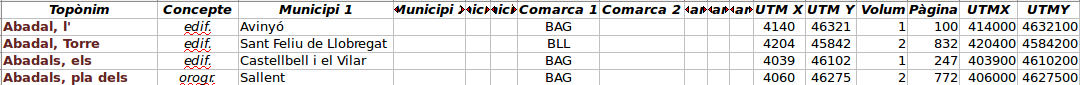
\includegraphics[height=2cm,width=16cm]{nomenclator_taula.png}
\caption{Fitxer excel amb les dades del Nomenclàtor oficial de toponímia major de Catalunya.}
\end{figure}
\subsubsection*{Neteja de les dades}
Ara que ja sabem el format que tenen les dades, ja podem iniciar el procés per a extreure la informació que ens interessa i deixar-la apunt per a ésser manipulada.\\
Per a fer aquest procés utilitzarem la llibreria \emph{xlrd} per a python, la qual ens permet la manipulació de fitxers amb dades procedents del Microsoft Excel, més concretament ens permet l'extracció de dades de fitxers d'Excel .xls i .xlsx a partir de la versió 2.0.\\ \\
De totes les dades que disposa la base de dades, es conservaran les dades referents al nom del municipi (columna "Topònim"), al tipus de municipi (columna "Concepte") i les seves coordenades geogràfiques corresponents a les columnes UTMX i UTMY.\\
Per a les dades corresponents a les coordenades, es convertiran aquestes dades al sistema de coordenades esfèriques, on mantindrem els paràmetres de latitud i longitud en la nostra base de dades.
\subsubsection*{Conversió de coordenades UTM a coordenades esfèriques (lat, lon)}
La conversió entre coordenades UTM i coordenades esfèriques (lat, lon), no és una feina senzilla, ja que aquesta conversió radica en diferents sistemes de representar el món. Per a poder realitzar la conversió es realitzen diferents operacions algebraiques que involucren operacions hiperbòliques i múltiples passos en funció de la zona UTM on vulguem fer aquest canvi. És per això que el primer que es necessita saber per a fer el canvi de coordenades és en quina zona es troba el punt que es desitja convertir. Les dades que es desitgen convertir són coordenades totes situades dins de Catalunya, i per tant mirarem en el mapa de zones UTM quina és la que pertoca.
\begin{figure}[htbp]
\centering
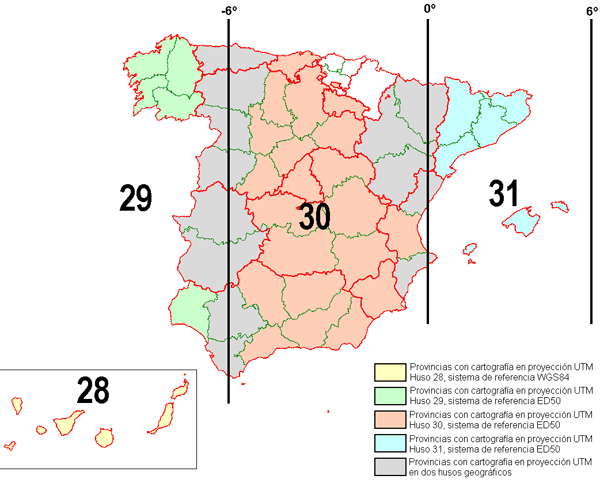
\includegraphics[width=9cm]{utm.png}
\caption{Mapa amb les zones UTM.}
\end{figure}
\newpage
Com es pot comprovar, la zona corresponent a Catalunya és la 31. Ara es necessita saber la lletra corresponent a la zona, que per a Catalunya és la 'T'.\\
Partint que per a la conversió, qualsevol coordenada dins de Catalunya tindrà com a zona la 31T, ja es pot fer servir una llibreria que ens permetrà la conversió de forma automàtica sense majors complicacions. S'utilitzarà la llibreria \emph{UTM}, i més concretament la seva funció to latlon().

\begin{figure}[!htbp]
\begin{verbatim}
coordenades = utm.to_latlon(item['utmX'],item['utmY'],31,'T')
item['lat'] = coordenades[0]
item['lon'] = coordenades[1]
\end{verbatim}
\caption{Conversió entre coordenades UTM i latitud/longitud.}
\end{figure}
Aquesta funció, com es pot veure a la figura anterior, retorna un vector amb primer el valor de la latitud, i després el corresponent a la longitud.\\ \\
Una vegada ja es tenen totes les dades que es desitgen pel projecte, es recorre tot el fitxer .xlsx que conté la informació de l'ICC i per cada fila es van agafant els valors especificats anteriorment. Es fa la conversió de les coordenades, i finalment cada valor es guarda a la base de dades amb l'\emph{insert} especificat anteriorment.
\newpage
\subsection*{Base de dades de ciutats de tot el món}
El treball es centra en una base de dades de notícies escrites en català i d'àmbit nacional, és per això que s'ha fet especial èmfasi en cobrir el territori català amb detall, però a nivell mundial s'ha optat per considerar només les ciutats més poblades.\\
Trobar una base de dades fiable i que reunís els requisits demanats consistia en tenir informació sobre les coordenades de cada ciutat, i a més informació sobre la seva població, ja que sinó no se'n podria determinar quina ciutat és suficientment important per a ésser considerada.\\ \\
La base de dades que s'ha escollit, ha estat la que manté geonames.org. Conté informació que es va actualitzant dia a dia, ja que tot i que el nucli d'aquesta informació prové de fonts oficials,  pot contenir errors i una comunitat activa de tot el món la va actualitzant i millorant. Aquesta base de dades és de lliure accés i ús sota una llicència Creative Commons.\\
La pàgina per accedir a les descàrregues de la base de dades, així com altres fitxers d'informació geogràfica diversa, es troba en el següent enllaç:

\begin{quote}
http://download.geonames.org/export/dump/
\end{quote}
Si observem els diferents fitxers que se'ns facilita a l'enllaç, podrem comprovar com n'hi ha de diferents tipus. Els fitxers que es poden trobar són:
\begin{itemize}
\item \textbf{XX.zip}: Conté informació per cada país, on XX correspon al seu codi ISO.
\item \textbf{allCountries.zip}: Tots els països en un sol fitxer.
\item \textbf{cities1000.zip}: Totes les ciutats amb una població major a 1000 habitants.
\item \textbf{cities5000.zip}: Totes les ciutats amb una població major a 5000 habitants.
\item \textbf{cities15000.zip}: Totes les ciutats amb una població major a 15000 habitants o capitals.
\item \textbf{alternateNames.zip}: Conté dos fitxers: el primer que conté els noms alternatius d'una ciutat (i.e.: el nom de la ciutat en diferents idiomes, noms alternatius d'una ciutat,...); el segon, és un fitxer que conté les referències entre els codis ISO i l'idioma que representen (i.e.: el català està representat amb el codi CA o CAT)
\item \textbf{admin1CodesASCII.txt}: Codis que fan referència a regions administratives en codificació ASCII.
\item \textbf{admin2Codes.txt}: Codis que fan referència a regions administratives en codificació UTF-8.
\item \textbf{iso-languagecodes.txt}: Codis ISO dels diferents idiomes. És el mateix fitxer inclòs dins del fitxer zip alternateNames.zip.
\item \textbf{featureCodes.txt}: Nom i descripció d'una característica. (i.e.: per a una entitat política es representa de la següent forma: "\emph{A.PCL	political entity}").
\item \textbf{timeZones.txt}: Informació sobre les hores de cada capital d'estat, concretament el desplaçament horari respecte DST i respecte el meridià de Greenwich.
\item \textbf{countryInfo.txt}: Informació diversa sobre cada país, com per exemple els codis postals o els idiomes oficials.
\item \textbf{...-<date>.txt}: Conté informació sobre les modificacions i eliminacions respecte l'anterior versió en cada un dels fitxers.
\item \textbf{Altres}: Hi ha altres fitxers que contenen informació com per exemple els autors de les modificacions.
\end{itemize}
Com s'ha mencionat anteriorment, es desitjarà mantenir una base de dades amb les ciutats més importants, i tal com podem veure hi ha fitxers que només contenen informació de les ciutats amb un nombre mínim d'habitants. En aquest cas, s'utilitzarà la base de dades amb ciutats que tenen una població superior als 15.000 habitants, per tant el primer fitxer a tenir en compte serà cities15000.zip i el fitxer alternateNames.zip per a poder agafar de cada ciutat el seu nom en català.\\
A continuació s'analitzarà l'estructura dels dos fitxers per a determinar quines són les propietats que desitgem extreure de cada un.\cite{geonames}
\subsubsection*{Estructura de les dades}
Cada fitxer de geonames.org està formatat de la mateixa manera: separant els camps amb tabulacions i amb codificació UTF-8.\\
\newpage
\subsubsection*{Taula 'Geonames'}
El fitxer cities15000.txt està estructurat seguint l'ordre dels camps marcats per la taula 'Geoname'.\cite{geonames}\\
\begin{itemize}
\item \textbf{geonameId}: Id en format enter
\item \textbf{name}: Nom del punt geogràfic en codificació UTF-8. És un varchar(200).
\item \textbf{asciiName}: Nom del punt geogràfic en format ASCII. És un varchar(200).
\item \textbf{alternateNames}: Diferents noms, separats per una coma, en format ASCII. És un varchar(10000).
\item \textbf{latitude}: Latitud en graus decimals (wgs84\footnote{El WGS84 és un sistema de coordenades cartogràfiques mundial que permet localitzar qualsevol punt de la Terra (sense necessitar cap altre punt de referència) per mitjà de tres unitats donades. WGS84 són les sigles en anglès de World Geodetic System 84 (Sistema Geodèsic Mundial de l'any 1984). S'estima un error de càlcul menor a 2 cm, per la qual cosa és utilitzat en el Sistema de Posicionament Global (GPS).}).
\item \textbf{longitude}: Longitud en graus decimals (wgs84).
\item \textbf{feature class}: Indica la classe de característiques. És un char(1).
\item \textbf{feature code}: Indica el codi de la característica. És un varchar(10).
\item \textbf{country code}: Codi de 2 lletres ISO-3166 del país. És un char(2).
\item \textbf{cc2}: Codis alternatius del país. Separat per comes. És un varchar(200).
\item \textbf{admin1 code}: Codi FIPS per identificar l'Estat. El codi '00' fa referència a països que no utilitzen el codi FIPS.
\item \textbf{admin2 code}: Codi per identificar la regió administrativa de segon nivell.
\item \textbf{admin3 code}: Codi per identificar la regió administrativa de tercer nivell.
\item \textbf{admin4 code}: Codi per identificar la regió administrativa de quart nivell.
\item \textbf{population}: Població de la ciutat. Format BigInt(enter de 8 bytes).
\item \textbf{elevation}: Alçada a la que es troba la ciutat. És un enter que correspon als metres.
\item \textbf{dem}: DEM (Digital Elevation Model), correspon a la representació 3D del territori. Aquest valor mostra la mitja d'alçada de la zona. És un enter que representa els metres.
\item \textbf{timezone}: Id de la zona horària a la que pertany la ciutat.
\item \textbf{modification date}: Data de la última modificació de la informació. En format yyyy-MM-dd.
\end{itemize}

\subsubsection*{Taula 'Alternate Names'}
El segon fitxer que s'utilitzarà per a identificar les ciutats d'arreu del món, és el que correspon a la representació dels noms de les ciutats en diferents idiomes. Aquest fitxer és l'anomenat \emph{alternatenames.txt}.\\
L'estructura d'aquest fitxer és la següent:
\begin{itemize}
\item \textbf{alternateNamesId}: La id d'aquest nom alternatiu. Enter.
\item \textbf{geonameId}: Id que fa referència a la taula 'Geoname'.
\item \textbf{isoLanguage}: Codi ISO 639 de l'idioma (2 o 3 caràcters); 'POST' per a codis postals; 'IATA', 'ICAO' i 'FAAC' fan referència a codis d'aeroports; 'FR 1793' fa referència a noms relacionats amb la Revolució Francesa; 'ABBR' per a abreviacions; 'LINK' fa referència a enllaços a pàgines web. És un varchar(7).
\item \textbf{alternate name}: Nom alternatiu o variant del nom. És un varchar(200).
\item \textbf{isPreferredName}: Serà '1' si aquest nom és l'oficial o el d'ús preferent.
\item \textbf{isShortName}: Serà '1' si és el nom abreviat, com podria ser 'Califòrnia' per fer referència a 'Estat de Califòrnia'.
\item \textbf{isColloquial}: Serà '1' si el nom s'utilitza normalment de forma col·loquial.
\item \textbf{isHistoric}: Serà '1' si el nom fa referència a un nom utilitzat en el passat, si és un nom històric.
\end{itemize}
S'ha de tenir en compte que la taula 'Geoname' conté un camp 'Alternate names', el qual és una versió reduïda de la informació que es pot trobar en el fitxer 'Alternate names'.
\\\\
Es manté informació sobre cada continent també, on els seus respectius codis seran:
\begin{table}[htbp]
\begin{center}
	\centering
    \begin{tabular}{| l | l | l | l |}
    \hline
    \textbf{Continent} & \textbf{Codi} \\ \hline
    AF: Àfrica &  geonameId = 6255146\\ \hline
	AS: Àsia & geonameId = 6255147\\ \hline
	EU: Europa & geonameId = 6255148\\ \hline
	NA: Amèrica del Nord & geonameId = 6255149\\ \hline
	OC: Oceania & geonameId = 6255151\\ \hline
	SA: Amèrica del Sud & geonameId = 6255150\\ \hline
	AN: Antàrtida & geonameId = 6255152\\ \hline
    \end{tabular}
\end{center}
\caption{Codis corresponents a cada continent.}
\end{table}
\newpage
\subsubsection*{Neteja de les dades}
Ara que ja s'han explicat els diferents paràmetres que contindrà cada fitxer, el primer pas és identificar tots els noms que hi ha disponibles en el fitxer alternateNames.txt en català.\\
Per a fer aquesta cerca, es recorrerà tot el fitxer mirant que el valor del paràmetre \emph{isoLanguage} sigui igual a '\emph{CAT}' o '\emph{CA}', que són les dues formes en què s'identifica la llengua catalana.\\
Una vegada es té aquesta informació, es farà ús de la llibreria \emph{json} disponible per a python, la qual ens permetrà guardar tots els registres que hem trobat en un fitxer amb format JSON per a poder-hi treballar de forma més còmode.\\
Tenint en compte que els diferents camps estan separats per tabulacions, la primera tasca serà diferenciar els diferents atributs d'una ciutat. Per a fer-ho utilitzarem la llibreria \emph{re}, una llibreria que ens permet fer operar amb expressions regulars. En aquest cas la operació és senzilla, només es vol separar un text segons les seves tabulacions:

\begin{figure}[!htbp]
\begin{verbatim}
textArray = re.split('\t+?',text)
\end{verbatim}
\caption{Ús de la llibreria \emph{re} per a separar un text segons les tabulacions.}
\end{figure}

La variable textArray, ara contindrà tota la informació relativa a una ciutat ordenada en un vector (i.e.: per a accedir a la ISO de l'idioma fariem textArray[2]).
\begin{figure}[!htbp]
\begin{verbatim}
with open('JSON/names.json', 'w') as fp:
    json.dump(llistaNoms, fp)
\end{verbatim}
\caption{Ús de la llibreria \emph{json} per a guardar una llista 'llistaNoms' en un fitxer en format JSON.}
\end{figure}

Es consideraran dos fitxers: el primer és \emph{names.json}, el qual conté la llista de noms disponibles en català (referent a la taula 'alternate names'); el segon és \emph{cites.json}, el qual contindrà la informació de totes les ciutats disponibles en el fitxer \emph{cities15000.txt}.\\
A continuació, el següent pas serà agafar tots els noms de ciutats disponibles en català (del fitxer names.json), i utilitzant la referència 'geonameId', trobar les dades de la ciutat que correspongui (del fitxer cities.json). Durant aquest procés, es descartaran les ciutats catalanes, ja que per al territori català es prioritzaran les dades obtingudes en la secció anterior, les de l'Institut Cartogràfic Català.\\
Fins aquest punt, es disposaran de dues bases de dades, la referent a Catalunya, i la referent a la resta del món.

\subsection*{Base de dades de notícies}
Per a l'obtenció de les dades referents a les notícies s'ha optat per a utilitzar els serveis RSS (Really Simple Syndication) que ofereixen alguns diaris catalans. El motiu és estrictament per comoditat i simplicitat. Per a aquest procés s'utilitzarà la llibreria \emph{BeautifulSoup} juntament amb  la llibreria \emph{feedparser} per a Python.\\
Aquest procés, el d'obtenir les notícies, s'ha d'anar executant cada cert temps, degut a que les notícies mitjançant RSS només estan disponibles durant un temps limitat, ja que el diari va renovant les notícies cada cert temps (normalment entre 1 i 2 dies). És per això, que per a automatitzar i simplificar el procés, s'ha decidit optar per implementar una tasca que s'executi cada certes hores. Per a l'automatització s'utilitzarà la llibreria \emph{twisted.internet} de Python.\\ \\

\subsubsection*{Obtenció d'un feed RSS}
La informació de les notícies s'obtindrà mitjançant RSS. Cada arxiu obtingut a través de RSS s'anomena feed (d'aquí ve el nom "\emph{feedparser}")\cite{feedparser}. Aquests arxius, estan definits a través d'estructures xml, que contindran una sèrie d'atributs predefinits per tal que aquests puguin ser descarregats desde aplicacions o gestors de RSS.\\
En el cas de les notícies proporcionades pel diari Ara, cada notícia té els següents atributs:

\begin{itemize}
\item \textbf{summary detail}: Resum de la notícia junt amb les imatges que pugui contenir, així com informació sobre l'idioma i l'enllaç a la pàgina web amb la notícia.
\item \textbf{published parsed}: Data de publicació de la notícia formatejat com a time struct.
\item \textbf{links}: Enllaços relatius a la notícia: l'enllaç web a la notícia pròpiament, i l'enllaç a les imatges que s'hi continguin. 
\item \textbf{title}: Títol de la notícia.
\item \textbf{tags}: Paraules clau que identifiquen la notícia.
\item \textbf{media thumbnail}: Enllaços a les imatges que acompanyin la notícia, així com les seves característiques bàsiques (per exemple la seva amplada i l'alçada).
\item \textbf{summary}: Resum de la notícia amb format html juntament amb la imatge que l'acompanyi.
\item \textbf{description}: Conté el cos de la notícia barrejat amb el codi html que l'hi dona format.
\item \textbf{content}: Subtítol de la notícia.
\item \textbf{guidislink}: És un booleà que en cas de ser cert, indica que es pot utilitzar el GUID\footnote{GUID: Identificador Únic Global.} com a enllaç de la notícia.
\item \textbf{title detail}: Títol de la notícia juntament amb altra informació com pot ser l'idioma de la notícia, o l'enllaç web.
\item \textbf{href}: Enllaços presents en la notícia.
\item \textbf{link}: Enllaç a la pàgina web on es pot trobar la notícia.
\item \textbf{published}: Data de publicació de la notícia en format String.
\item \textbf{media content}: Informació a tots els arxius multimèdia (fotos, vídeos, àudios,...) presents en la notícia.
\item \textbf{id}: Identificador de la notícia. En aquest cas coincideix amb el valor especificat a l'apartat \emph{Link}.
\item \textbf{media keywords}: Paraules claus que identifiquen la notícia.
\end{itemize}
En el projecte ens interessen especialment els camps de Títol, la data de publicació i el cos de la notícia que podríem trobar en el camp de summary, però que com s'explicarà a continuació, la agafarem fent servir un altre llibreria, BeautifulSoup.
\subsubsection*{Formatació del text de la notícia}
La informació del cos de la notícia present en els camps que hem vist anteriorment, conté codi html barrejat. És per això, que s'ha decidir utilitzar la llibreria BeautifulSoup.\\
Aquesta llibreria, ens permet separar el codi html de la resta de text, d'una forma similar a com fariem servir un diccionari en python. Per exemple, tenim el següent codi HTML:

\begin{figure}[!htbp]
\begin{verbatim}
<title>
	Això és un títol!
</title>
\end{verbatim}
\end{figure}
Fent servir BeautifulSoup, si desitgéssim obtenir el títol en qüestió, és a dir "Això és un títol!", hauríem de fer senzillament:

\begin{figure}[!htbp]
\begin{verbatim}
soup = BeautifulSoup(documentHTML)
soup.title.string
# Això és un títol!
\end{verbatim}
\end{figure}
Aquest codi ens retornaria el text desitjat.\\
Així doncs, per a obtenir el text de la notícia agafarem l'atribut description del feed RSS, i utilitzant BeautifulSoup\cite{beautifulsoup} ens quedarem amb el text només. I el mateix per al títol.	
\begin{figure}[!htbp]
\begin{verbatim}
 title = BeautifulSoup(key["title"]).get_text()
 description = BeautifulSoup(key["description"]).get_text()
\end{verbatim}
\caption{Obtenció del títol i el cos d'una notícia mitjançant BeautifulSoup i feedparser.}
\end{figure}
\subsubsection*{Formatació de la data de publicació}
Per a guardar la data relativa a la publicació de la notícia també la haurem d'adaptar, per tal que pugui ser utilitzada més endavant com a referència temporal. Per a fer-ho, utilitzarem la llibreria \emph{time} juntament \emph{datetime}.\\
Si analitzem el que ens retorna el paràmetre "published parsed" del RSS, veiem que el seu valor té el següent format\cite{rss}
\begin{figure}[!htbp]
\begin{verbatim}
time.struct_time(tm_year=2015, tm_mon=6, tm_mday=22, tm_hour=22, tm_min=0, 
tm_sec=0, tm_wday=0, tm_yday=173, tm_isdst=0)
\end{verbatim}
\end{figure}

Com podem veure, el format que ens retorna no ens és apte per a ser manipulat encara, i és per això que farem servir la funcio \emph{mktime} de la llibreria time, la qual ens convertirà la data en "Epoch time", és a dir en els segons que hi ha entre la data a analitzar i l'1 de gener de 1970. En aquest cas ens retornaria el següent float: 1435006800.0. Com que tampoc es desitja tenir la data en segons, s'utilitzarà la llibreria \emph{datetime}, i més concretament la funció \emph{fromtimestamp}, la qual ens retornarà la data amb la formatació adequada\cite{time}. 

\begin{figure}[!htbp]
\begin{verbatim}
seconds_since_epoch = mktime(key["published_parsed"]
print datetime.fromtimestamp(mktime(seconds_since_epoch))
# 2015-06-22 23:00:00
\end{verbatim}
\end{figure}

En aquest punt, tota la informació de la notícia ja està apunt per a ésser desada a la base de dades.
\subsubsection*{Automatització del procés d'obtenció de notícies}
El procés d'obtenció de notícies és una tasca que s'ha d'anar realitzant regularment, i és per això que s'ha optat per a automatitzar el procés utilitzant la llibreria \emph{twisted.internet}. L'objectiu serà que cada cert temps s'executi una funció que obtingui la informació utilitzant els mètodes anteriorment descrits, i guardi tota la informació de cada notícia en una base de dades.\\
L'ús de la llibreria resulta molt senzill, i senzillament, considerant que la funció que obté les notícies en un moment donat s'anomena \emph{getNewsJob()}, i considerant que es vulgui executar el procés cada 6 hores (al projecte s'ha realitzat l'obtenció cada 24h) s'hauria d'implementar el següent codi:
\newpage
\begin{figure}[!htbp]
\begin{verbatim}
from twisted.internet import task
from twisted.internet import reactor

hours = 6 # the job will run every 6 hours
timeout = hours*60.0*60.0 # Sixty seconds * num of minutes
def doWork():
    get_news_job()
    pass

l = task.LoopingCall(doWork)
l.start(timeout) # call every six hours

reactor.run()
\end{verbatim}
\end{figure}

Una vegada creat aquest codi, s'ha creat fitxer separat del document IPython i s'ha posat com a procés que s'executa cada vegada que s'engega l'ordinador (s'executa en engegar l'ordinador, i si aquest no s'ha tancat, s'executarà al cap de 24h).

\subsection{Obtenció de localitats en un text}
La següent etapa del procés, consisteix en analitzar la base de dades de notícies de la que es disposa, per a poder identificar en el text (ja sigui el títol o el cos de la notícia) les localitats amb referències geogràfiques.\\
Aquest procés, al no disposar d'una base de dades d'entrenament, s'ha hagut de realitzar a base d'identificar les característiques que solen tenir els noms de ciutats en un text en català.\\
El primer pas ha estat crear dues llistes amb les paraules clau que ens permetran identificar una possible localitat en un text. Aquestes llistes, es crearan per evitar haver de fer consultes constantment a cada paraula trobada. La primera llista pertany a les localitats catalanes, i la segona a les de la resta de món.\\
Una paraula clau, serà la primera paraula que comenci amb majúscula (es descarten articles inicials) del nom de la localitat. Per exemple, si considerem el nom de \emph{les Borges Blanques}, la paraula clau seria \emph{Borges}. Aquest enfocament es pot fer, ja que els articles en la base de dades, estan sempre escrits en minúscula.\\\\
A continuació, s'ha creat un diccionari, on es guardarà per cada paraula clau, el nombre mínim i el màxim de paraules que formen el nom d'una localitat que comença per la paraula clau en qüestió. Per exemple, tenim la paraula clau \emph{Abella}. A Catalunya hi ha dues ciutats que comencen amb aquesta paraula clau, \emph{Abella} i \emph{Abella de la Conca}. El que es guardaria en aquest diccionari seria la paraula clau \emph{Abella} i la longitud mínima, que és una paraula (\emph{Abella}), i la longitud màxima, que seria 4 (\emph{Abella de la Conca}). I així, per a totes les paraules clau de Catalunya i també per a les de la resta del món.\\
Com a dada es pot veure que per a les localitats catalanes els valors oscil·len entre un mínim d'una paraula i un màxim de 5, mentre que per la resta del món, oscil·len entre un mínim d'una paraula i un màxim de 7 paraules.\\\\
Per a començar el procés d'identificació de localitats, es pressuposarà que el periodista que ha escrit la notícia, haurà escrit el nom de la localitat correctament, és a dir, que la cerca de ciutats serà sensible a majúscules i minúscules.\\
Per a evitar errors al buscar localitats es mantenen tres llistes, una que contindrà una llista d'articles, una altra que contindrà noms de persona, i una tercera que contindrà una llista negra de localitats.\\
Per cada notícia el procés serà el mateix, i seguirà el següent esquema:
\begin{enumerate}
\item Si la paraula comença amb majúscula i està dins una llista negra, s'ignora. La llista negra contindrà paraules que són ciutats que rarament apareixen en notícies de Catalunya, però que no obstant poden coincidir amb paraules o noms que si que es repeteixen freqüentment. Això es fa per evitar el màxim possible els falsos positius de ciutats, amb casos com el poble de "\emph{Les}" a la Vall d'Aran, o la ciutat de "\emph{Un}" a la Índia, o casos que es podrien confondre amb cognoms que són ciutats i que es repeteixen molt als diaris però que aquesta importància no correspon amb la importància del poble. Com a exemple podriem tenir la petita ciutat de "Montilla" a Andalusia.
\item Si la paraula anterior o aquesta comencen amb majúscula i a més es troben dins de la llista de noms de persona, s'ignora. Les llistes de noms que es tenen són: una amb noms de persona en català\cite{softcatala}, i una de global\cite{nomsmon}. D'aquesta manera s'evita que noms o cognoms de persona es confonguin amb localitats.
\item Si la paraula comença amb majúscula i està dins la llista de paraules clau es fa el següent:
\begin{enumerate}
\item Si s'ha arribat aquí, vol dir que tenim una possible localitat candidata. Per tant, en aquest punt, guardarem la paraula clau, junt amb tantes paraules posteriors com indiqui el valor màxim del diccionari que hem mencionat anteriorment, el qual conté les longituds dels noms de localitats relacionats amb la paraula clau.
\end{enumerate}
\item En aquest moment, es té una llista de possibles candidates, per a tractar els resultats es seguirà el següent procés:
\begin{enumerate}
\item Com que de cada paraula clau s'ha guardat la paraula, a més de les paraules del costat que poden formar una localitat, començarem mirant les frases més llargues i anar reduint cada vegada una paraula fins a trobar alguna localitat vàlida. Per exemple:
\begin{itemize}
\item Donada la paraula clau \emph{Abella}, i tenint que la longitud màxima que forma un nom de localitat és 4, i el mínim és 1, s'agafen les 3 paraules que apareixen després de \emph{Abella}. Tenim el grup de paraules [\emph{Abella, és, un, poble}], amb una longitud de 4 paraules, ja que és la longitud màxima que tenim al diccionari. Començarem mirant la frase més llarga, en aquest cas \emph{Abella és un poble}, en comprovar si aquesta localitat està a la llista de localitats, veurem que no hi és. El procés segueix comprovant successivament fins a trobar una localitat vàlida, primer mirarà amb longitud 3 \emph{Abella és un}, al no trobar-la tampoc, seguirà amb \emph{Abella és} i finalment \emph{Abella}. Finalment haurà trobat que \emph{Abella} si que és un poble i l'afegirà a les localitats trobades.
\end{itemize}
\item Les localitats trobades es guardaran en una llista. Fins ara, el procés de cerca de ciutats no ha fet cap consulta a base de dades.
\end{enumerate}
\end{enumerate}
 
\subsection{Obtenció de les coordenades d'una localitat}
Una vegada es té una llista amb les paraules que hem identificat com a localitats, es fan les crides corresponents a la base de dades per a obtenir la informació relativa a cada una.\\
Obtenir les coordenades, una vegada ja es tenen els noms de les localitats, és tan simple com fer una consulta en una base de dades. Per tant, ara només cal fer aquestes consultes per cada ciutat trobada i guardar-ne les dades en una variable per a procedir al següent pas.
\subsection{Formatació de les dades per a CartoDB}
Per a la visualització de les dades en un mapa, s'ha escollit el servei de software web (Software As A Service - SAAS) CartoDB. Aquest sistema, ens permetrà representar les dades utilitzant les dades de geolocalització (latitud i longitud) que contindrà la nostra base de dades de resultats. Abans d'això, haurem de donar el format correcte a les nostres dades, ja que CartoDB accepta un format concret de JSON, però per desgràcia el format que s'ha provat com a resultat d'aquest projecte, no ha funcionat correctament. Com que també accepta el format CSV, donarem aquest format a la sortida de les dades del projecte.\\
\\
Per a poder fer aquest pas farem servir la llibreria \emph{CSV} de Python. El procés serà senzill, l'únic que haurem de fer és anar escrivint cada element de la llista de resultats en el fitxer CSV resultant, de la següent forma:

\begin{figure}[!htbp]
\begin{verbatim}
import csv
from bson import json_util
with open('CSV/found_cities.csv', 'wb') as f:
    w = csv.writer(f,delimiter=',')
    for a in range(len(lst)):
        w.writerow(lst[a])
\end{verbatim}
\end{figure}

Una vegada el procés ha finalitzat ja tenim les dades a punt per a pujar-les a CartoDB i visualitzar-les.
\subsection{Aplicació de l'algorisme DBScan}
Per a proporcionar una vista opcional de les dades, amb menys punts geogràfics, on es podran agrupar les coordenades que resultin properes, s'utilitzarà l'algorisme de clustering DBScan.\\
Aquest algorisme clusteritza les dades basant-se amb dos paràmetres: una distància física entre els diferents punts, i la mida mínima del clúster. Farà créixer un clúster, sempre i quant la densitat en aquesta zona sigui suficientment alta. El funcionament és el següent:
\begin{itemize}
\item Busca clústers mirant el veïnat de cada punt determinat per la distància èpsilon especificada com a paràmetre.
\item Si en el veïnat d'un punt hi ha més del mínim de punts especificats per la variable \emph{minPunts}, es crearà un nou clúster amb el punt analitzat com a centre.
\item Iterativament l'algorisme anirà recol·lectant els punts que són directament assolibles des dels centres dels clústers.
\item El procés acabarà quan ja no es poden afegir nous punts a cap clúster.
\end{itemize}
Per a adaptar aquest algorisme al projecte, s'utilitzaran les llibreries disponibles en les llibreries \emph{panda}, \emph{sklearn.cluster}, \emph{geopy.space}, \emph{numpy}, i per a visualitzar les dades de prova, s'utilitzarà la llibreria \emph{matplot.pyplot}\cite{panda}.\\
Primer, fent servir pandas, convertirem les dades obtingudes anteriorment en una matriu que tindrà per columnes els valors de la latitud i la longitud respectivament.\\
Fent servir la funcio DBSCAN de la llibreria sklearn.cluster aplicarem DBSCAN amb uns valors arbitraris, que en aquest cas considerarem que són 0.2 per la distància èpsilon, i 1 al mínim de valors per clúster.\\
Com a exemple del seu resultat i funcionament utilitzarem les coordenades de 5 localitats que es troben molt properes entre elles:

\begin{table}[!htbp]
\begin{center}
	\centering
    \begin{tabular}{| l | l | l | l |}
    \hline
    \textbf{Poble} & \textbf{Latitud} & \textbf{Longitud} \\ \hline
    Riba-roja d'Ebre & 41.252 &  0.489\\ \hline
	Flix & 41.813 & 0.92\\ \hline
	Amposta & 40.711 & 0.518 \\ \hline
	Ascó & 41.182 & 0.57\\ \hline
	Garcia & 41.14 & 0.652\\ \hline
    \end{tabular}
\end{center}
\caption{Localitats d'exemple per comprovar el funcionament de DBSCAN.}
\end{table}
En aplicar DBSCAN el primer que obtenim és el nombre de clústers que ha trobat, que en aquest exemple, ens n'ha retornat 3. El codi per obtenir el nombre de clústers i agrupar els clusters en una llista és el següent:
\newpage
\begin{figure}[!htbp]
\begin{verbatim}
num\_clusters = len(set(labels)) - (1 if -1 in labels else 0)
clusters = pd.Series([coordinates[labels == i] for i in xrange(num\_clusters)])
\end{verbatim}
\end{figure}
En el codi anterior, \emph{num\_clusters} representarà el nombre de clústers que es crearan, i la variable \emph{clusters} contindrà els diferents clústers trobats.\\
Ara, de cada clúster que s'ha trobat, es voldrà obtenir un punt, concretament buscarem el punt més proper al centroide del clúster, és a dir el punt que està més aprop del centre de les diferents coordenades del clúster.
\begin{figure}[htbp]
\centering
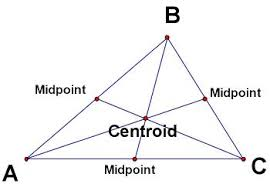
\includegraphics[width=5cm]{centroide.jpg}
\caption{Representació del centroide d'un triangle\cite{centroid}.}
\end{figure}

Per a trobar el centroide utilitzarem la següent fórmula, que donat un conjunt de punts retorna el punt centroide del clúster.
\begin{figure}[!htbp]
\begin{verbatim}
def getCentroid(points):
    n = points.shape[0]
    sum\_lon = np.sum(points[:, 1])
    sum\_lat = np.sum(points[:, 0])
    return (sum\_lon/n, sum\_lat/n)
\end{verbatim}
\end{figure}

Ara que ja tenim el clúster, hem de trobar el punt dels que disposem que sigui més proper al centroide. D'aquesta forma es tindran dues funcions, una anomenada \emph{getCentroid} que retornarà el centroide d'un conjunt de punts; i una altra que s'anomenarà \emph{getNearestPoint}, que donat un punt centroide, i una llista de punts, retornarà quin d'aquests punts s'aproxima més al centroide.\\ \\
Un cop es tenen les dues funcions, ja es pot aplicar l'algorisme per a trobar les coordenades centrals on es situaran els clústers. Per a fer-ho, declararem dues llistes, una de latituds i una de longituds, que contindran les posicions finals de cada clúster.\\
Donat que calcular el centroide de dos punts no té massa sentit, agafarem el primer d'aquests dos punts en cas que hi hagi dos o menys punts.\\
En qualsevol altre cas, si n'hi ha més de 2, aplicarem la funció que ens calcula el punt més proper al centroide (\emph{getNearestPoint}). D'aquesta manera ja tindrem les coordenades dels diferents centroides.

\begin{figure}[!htbp]
\begin{verbatim}
lon = []
lat = []
for i, cluster in clusters.iteritems():
    if len(cluster) < 3:
        representative_point = (cluster[0][1], cluster[0][0])
    else:
        representative_point = getNearestPoint(cluster, getCentroid(cluster))
    lon.append(representative_point[0])
    lat.append(representative_point[1])
    res_list.append([representative_point[1],representative_point[0]])
rs = pd.DataFrame({'lon':lon, 'lat':lat})
\end{verbatim}
\caption{Algorisme per aplicar DBSCAN.}
\end{figure}
\newpage
Utilitzant la llibreria matplotlib.pyplot mostrarem els resultats per veure els diferents clústers.

\begin{figure}[!htbp]
\centering
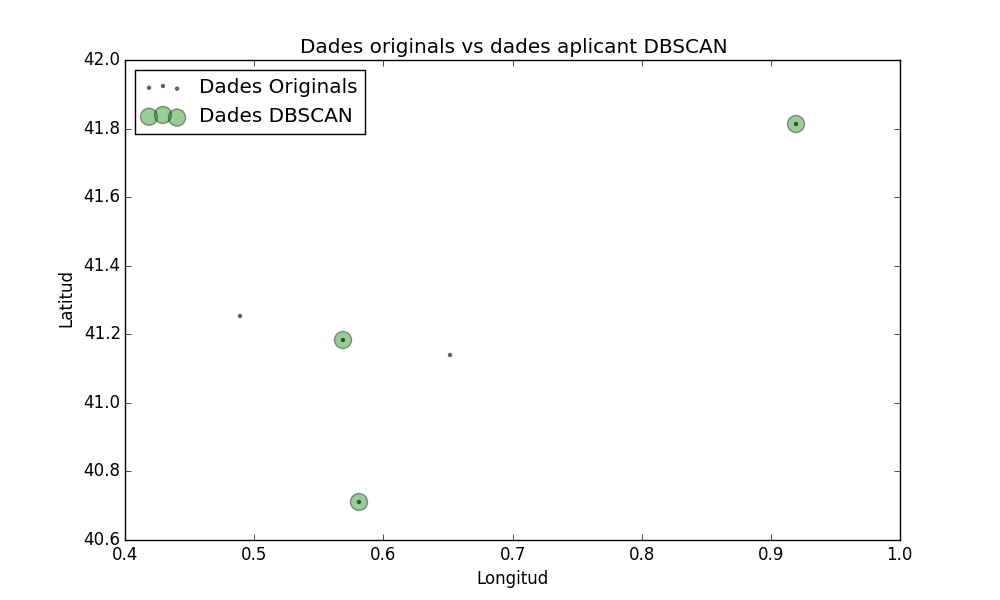
\includegraphics[width=8cm]{dbscan.png}
\caption{Exemple d'aplicació DBSCAN, donades 5 localitats properes.}
\end{figure}
Tal com es pot veure en la figura anterior, el resultat mostra tres clústers (els cercles grans) i els punts negres petits, són les posicions originals dels diferents pobles. D'aquesta manera en el mapa, els punts que estiguin propers no es mostrarien per separat.\\\\
Tot seguit s'aplicarà l'algorisme DBScan als resultats de la base de dades de notícies per a comprovar el resultat.
\begin{figure}[htbp]
\centering
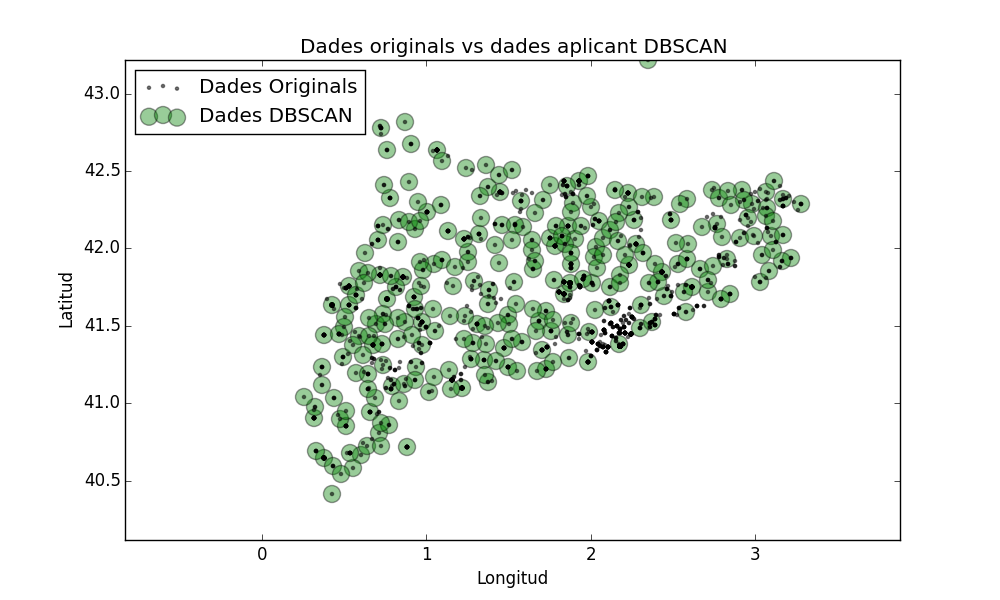
\includegraphics[width=12cm]{clustering-005-1.png}
\caption{DBScan en la base de dades de notícies, amb èpsilon 0.05.}
\end{figure}
Tal com es pot comprovar en la imatge, en aplicar DBScan amb una distància èpsilon de 0.01 es pot veure com quasi cada punt negre, que representen les referències localitzades en les notícies, i els cercles verds que indiquen els clústers finals. També es pot veure com tot i no haver-hi un mapa, es pot distingir perfectament la forma de Catalunya, donat que és la zona amb més presència de notícies en la base de dades.\\
\newpage
Si aquest valor èpsilon s'incrementa, s'espera que es creïn clústers més grans, i per tant, n'hi haurà menys quantitat. Per a comprovar-ho es provaran els valors de 0.1, 0.2.

\begin{figure}[htbp]
\centering
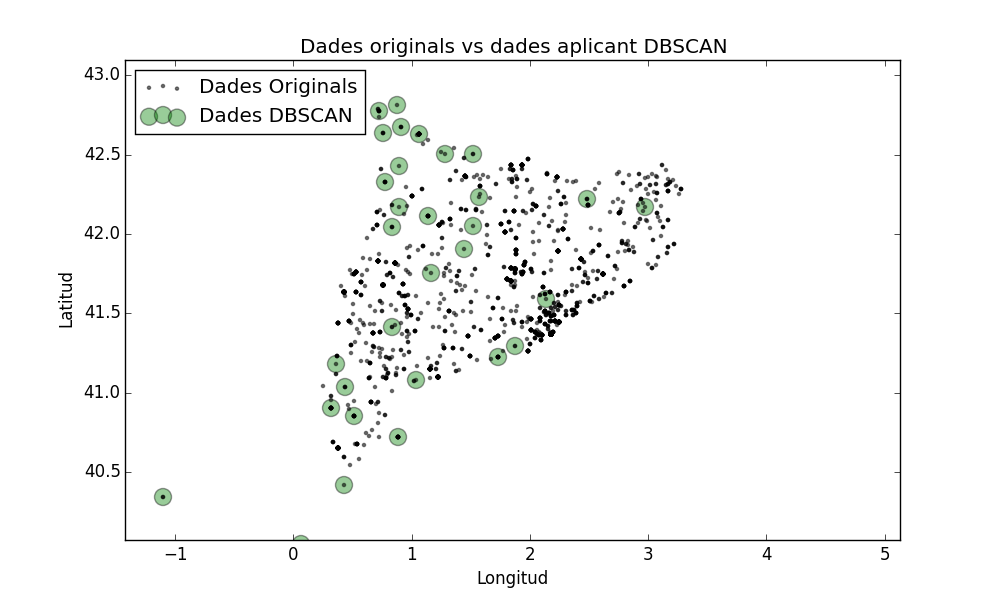
\includegraphics[width=7cm]{clustering-01.png}
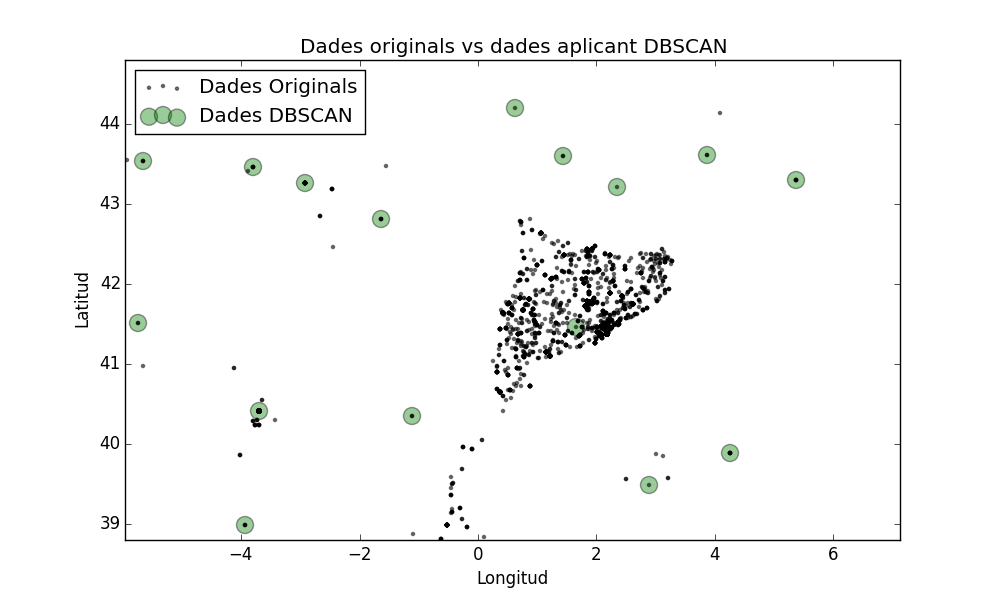
\includegraphics[width=7cm]{clustering-02.png}
\caption{DBScan en la base de dades de notícies, amb èpsilon 0.1 a l'esquerra i 0.2 a la dreta.}
\end{figure}
En les dues figures anteriors, es pot veure a l'esquerra la imatge corresponent a distància èpsilon 0.1, i es veu com ja hi ha molts menys clústers respecte a l'èpsilon amb valor 0.05. I a la dreta podem veure la imatge corresponent a un valor 0.2 de l'èpsilon i en aquest cas ja només queda un clúster per tot Catalunya\cite{dbscan}.
\newpage
\subsection{Visualització de les dades}
Per a visualitzar les dades de forma que es mostrin a sobre d'un mapa, i es puguin veure de forma interactiva les localitats que s'han obtingut de l'anàlisi anterior, s'utilitzarà CartoDB. Per a visualitzar les dades, és tan senzill com a registar-se a la pàgina web de cartodb.com, pujar les dades, i a continuació especificar quina columna de la nostra base de dades correspon a la longitud, quina a la latitud, i si s'escau, quina conté les dades temporals.\\
Una vegada les dades han estat correctament formatejades, ja podrem visualitzar un mapa bàsic amb els diferents punts pintats.\\
Per a mostrar la informació referent a la freqüència en què un punt ha estat trobat en la base de dades es farà servir el tipus de visualització \emph{CLUSTER}. Aquesta visualització aplica un clúster automàticament en funció del nivell de zoom aplicat. 

\begin{figure}[!htbp]
\centering
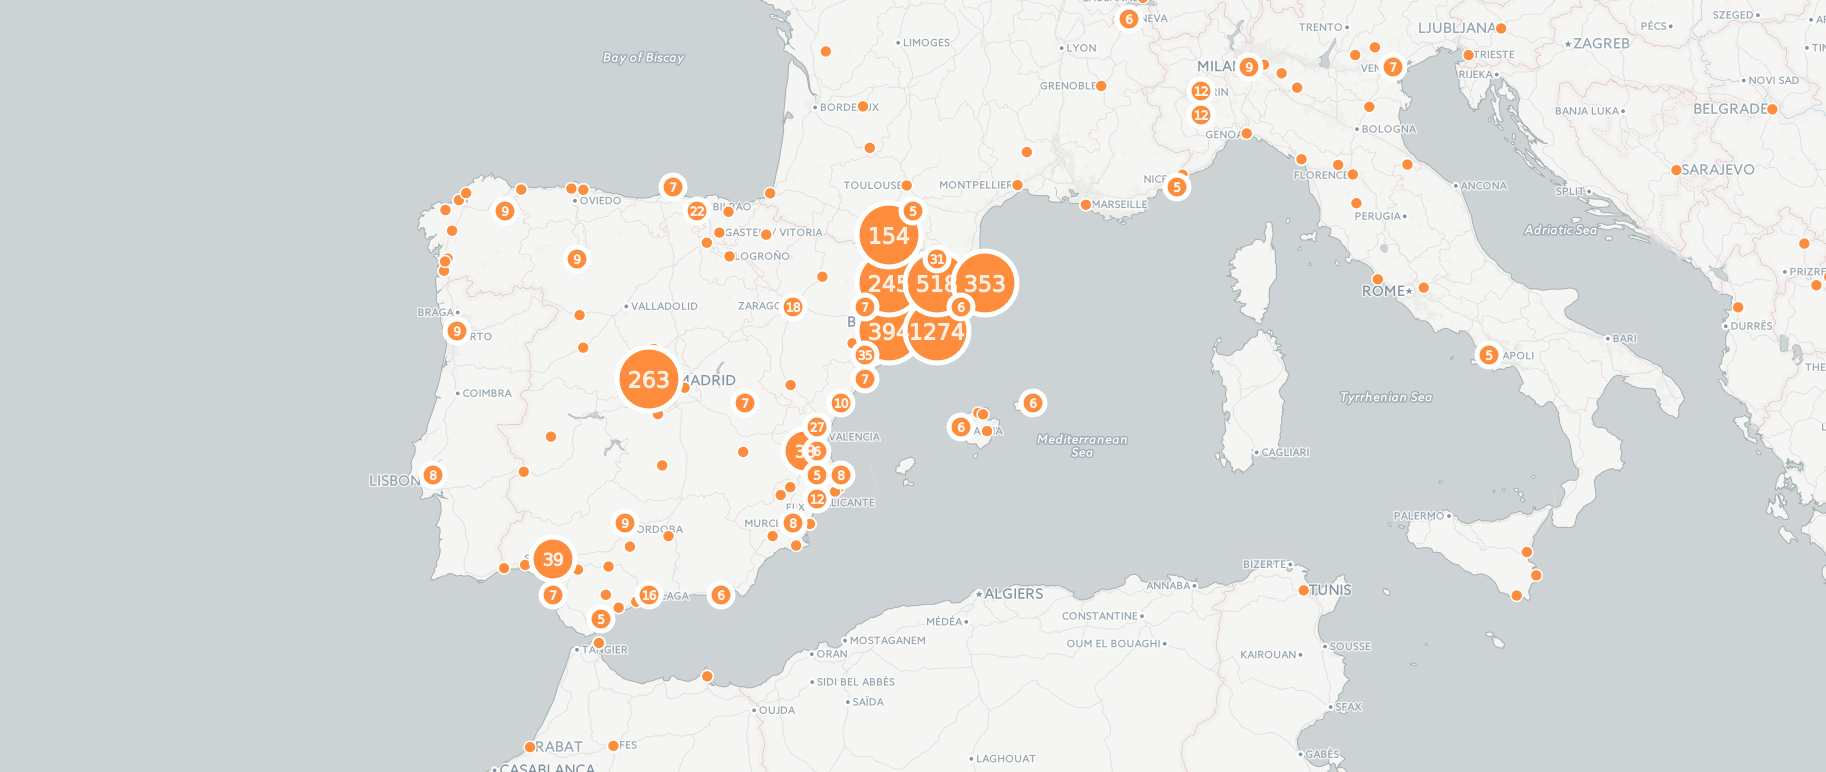
\includegraphics[width=12cm]{cartodb-1.png}
\caption{Visualització de les dades per a la zona de la península ibèrica, utilitzant el filtre CLUSTER de CartoDB.}
\end{figure}

La primera tasca un cop hem representat les dades és a simple vista si segueix una lògica la representació d'aquestes dades. En aquest cas es pot veure com a Catalunya hi ha una gran quantitat de notícies, concretament es pot veure a la zona de Barcelona un clúster amb una densitat de més de 1200, a la zona de Tarragona una densitat de vora 400, a Girona de poc més de 353, a la Catalunya central es veu una densitat de prop de 520 aparicions.\\
A Espanya es poden veure densitats inferiors, excepte a Madrid, que és la ciutat que concentra més referències de fora de Catalunya, amb una densitat de 263. La segona ciutat espanyola amb més representació és Sevilla, amb una densitat de 39 aparicions.\\ \\
Com s'ha explicat en la secció d'obtenció de les notícies, la base de dades del projecte també inclou un camp amb la data de publicació de cada notícia, i gràcies a aquesta opció, també podem considerar una altra opció de visualització, anomenada "Torque". Aquesta visualització ens permet especificar un camp de la base de dades, com a referència temporal, i una vegada definida, permet mostrar l'aparició de les diferents localitats en funció de la data.

\begin{figure}[!htbp]
\centering
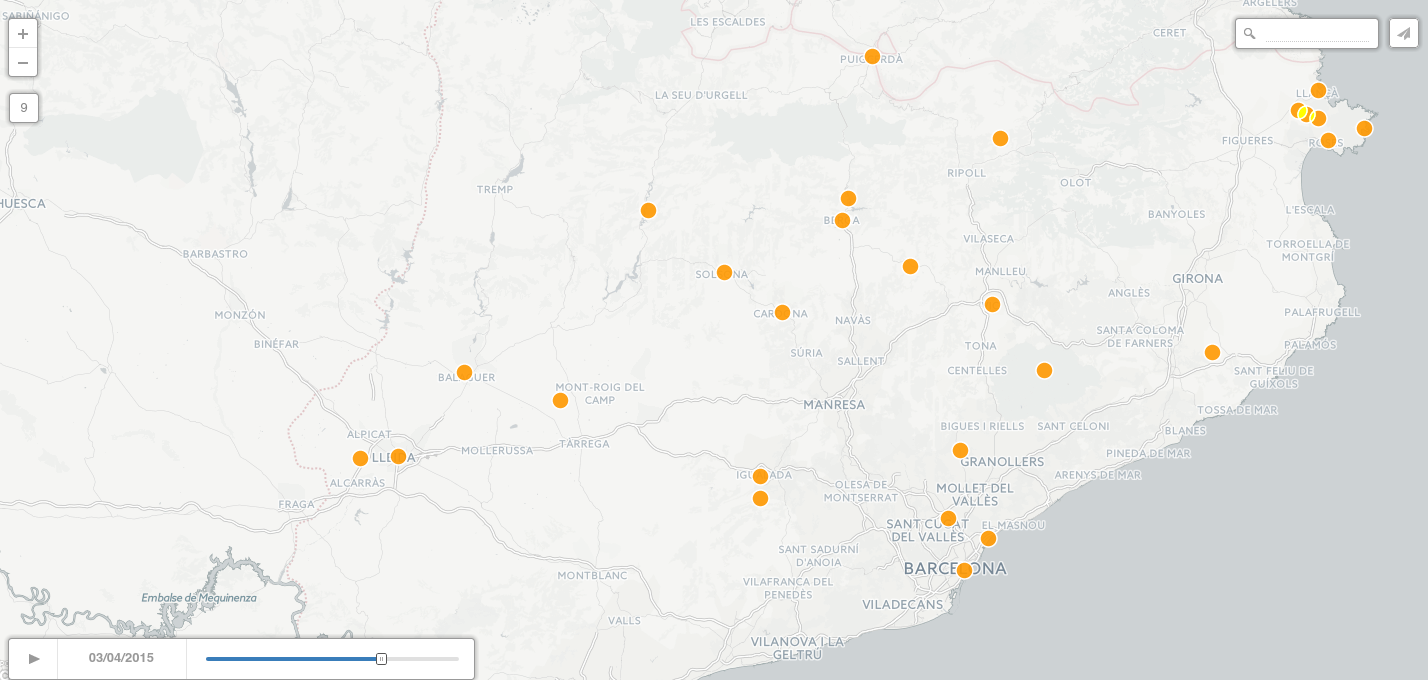
\includegraphics[width=12cm]{cartodb-2.png}
\caption{Visualització de les dades per a la zona de Catalunya, utilitzant el filtre TORQUE de CartoDB.}
\end{figure}
\newpage
Com a darrer exemple, i per comprovar un altre filtre, a més de comprovar si els resultats fora de Catalunya, tenen sentit, es mostraran els resultats relatius a Amèrica del Nord, utilitzant un mapa de calor, en què com més vermell sigui, més freqüència de notícies hi ha hagut, i per contra, el blau indica poca densitat. En cas que no tingui cap marca de color, senzillament indica que no ha aparegut a la base de dades.

\begin{figure}[!htbp]
\centering
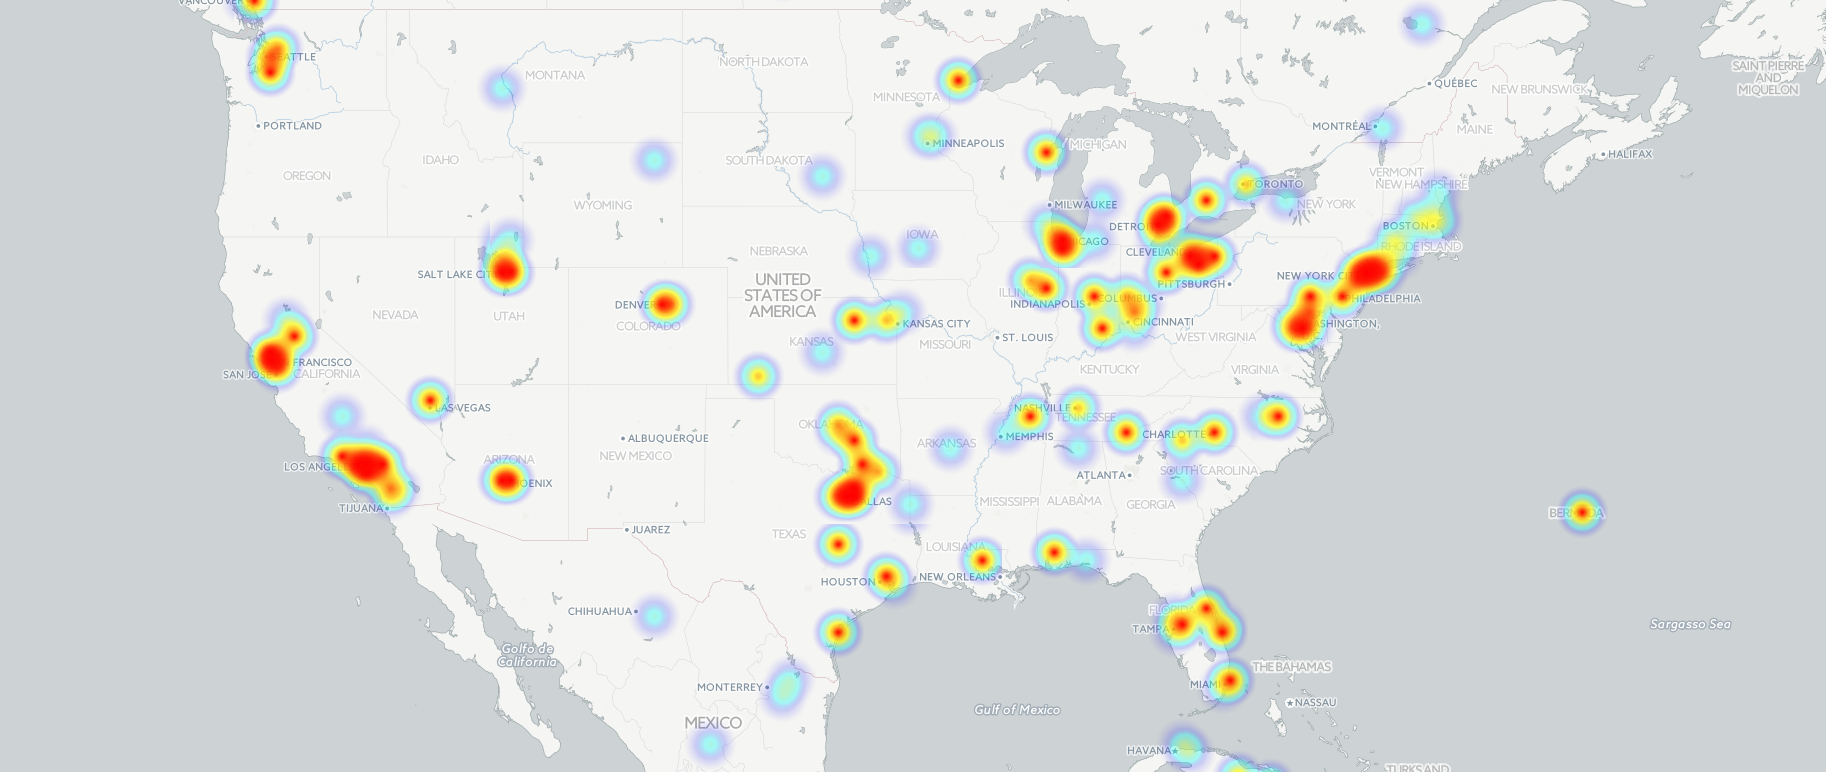
\includegraphics[width=12cm]{cartodb-3.png}
\caption{Visualització de les dades per a la zona dels Estats Units, utilitzant el filtre HEATMAP de CartoDB.}
\end{figure}

Com es pot veure a la imatge anterior, els resultats tenen sentit, ja que les zones amb més densitat són les principals ciutats d'Estats Units. A la costa Est hi ha una alta densitat a les ciutats de Nova York, Washington i Boston; tame hi ha una densitat important a Florida, concretament a les zones de Miami, Tampa i Deltona; al centre dels Estats Units destaca la zona de Dallas, de Denver i de Kansas City; en quant a la costa Oest, les principals zones a destacar són Seattle, San Francisco i Los Ángeles.\\
Per tant, aparentment els resultats estan indicant les principals ciutats del país, i això dóna sentit als resultats trobats.\\\\
Es faciliten 3 mapes preparats per a ser visualitzats. Aquests mapes estaran disponibles tant a la pàgina web alsolanes.github.io/TFG com al full IPython junt amb la resta de codi.\\
El primer full conté una visualització amb els resultats acumulats on es veu el clustering automàtic que aplica CartoDB, representant les zones amb més presència a les notícies amb clústers més grans.

\begin{figure}[!htbp]
\centering
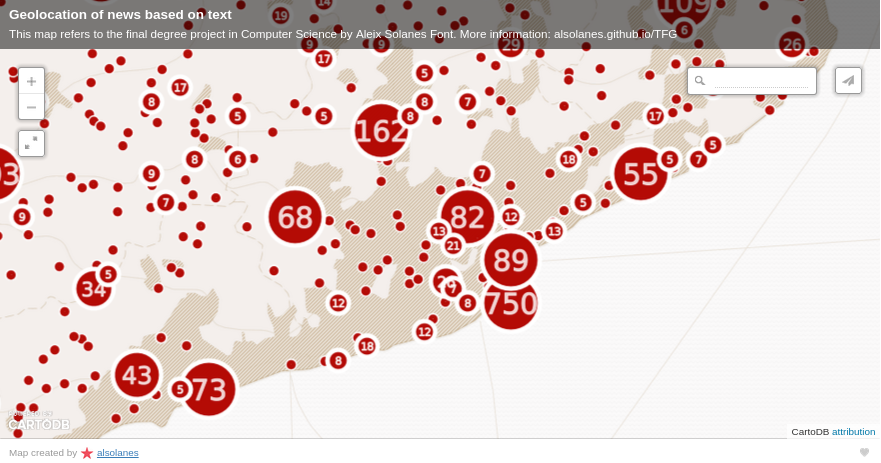
\includegraphics[width=12cm]{cartodb-res-1.png}
\caption{Mapa disponible per a la divulgació.}
\end{figure}

El segon mapa conté tres capes, les quals es poden escollir de visualitzar per separat.\\
La primera capa mostra l'acumulació total de referències, igual que el mapa anterior. La segona capa permet veure les referències geogràfiques separades segons el diari. I per últim permet veure l'evolució temporal, mostrant bombolles que apareixen el dia en què hi va haver una referència de la localitat.

\begin{figure}[!htbp]
\centering
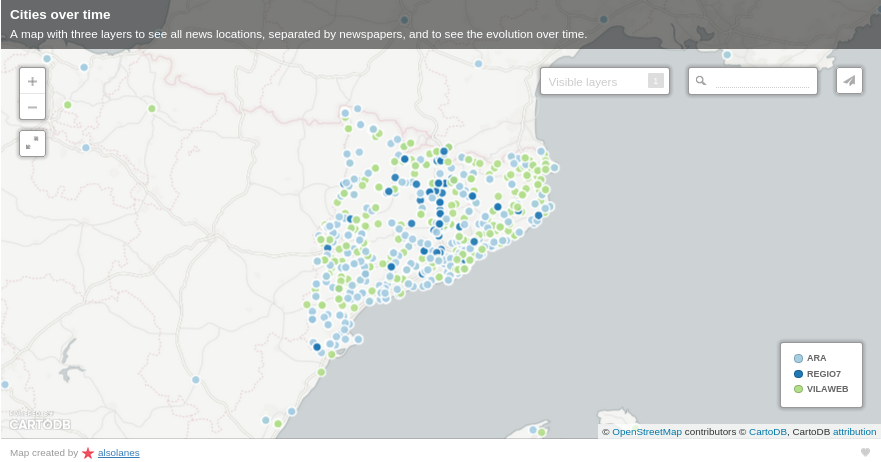
\includegraphics[width=12cm]{cartodb-res-2.png}
\caption{Mapa disponible per a la divulgació, es visualitza la capa amb les dades separades per diari.}
\end{figure}

També es facilita un mapa que mostra l'evolució acumulada de les aparicions de les referències geogràfiques. Aquest mapa correspon a un mapa de calor (Heat map), i permet veure l'evolució en funció del temps.

\begin{figure}[!htbp]
\centering
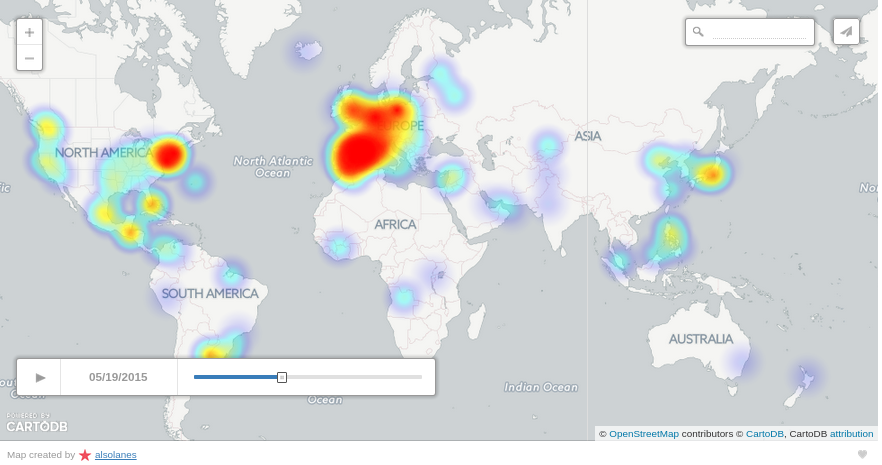
\includegraphics[width=12cm]{cartodb-res-3.png}
\caption{Mapa disponible per a la divulgació. Mapa de calor en funció del temps.}
\end{figure}

Finalment es mostra un mapa que conté 4 capes, cada una de les quals correspon a una distància èpsilon diferent. Com més gran sigui l'èpsilon, el clúster contindrà referències de més lluny, per tant a èpsilon més gran, menys clústers però més densos. En aquest mapa es permet veure els resultats d'aplicar clústering amb valors de èpsilon 0.05, 0.1, 0.2 i 0.8.
\begin{figure}[!htbp]
\centering
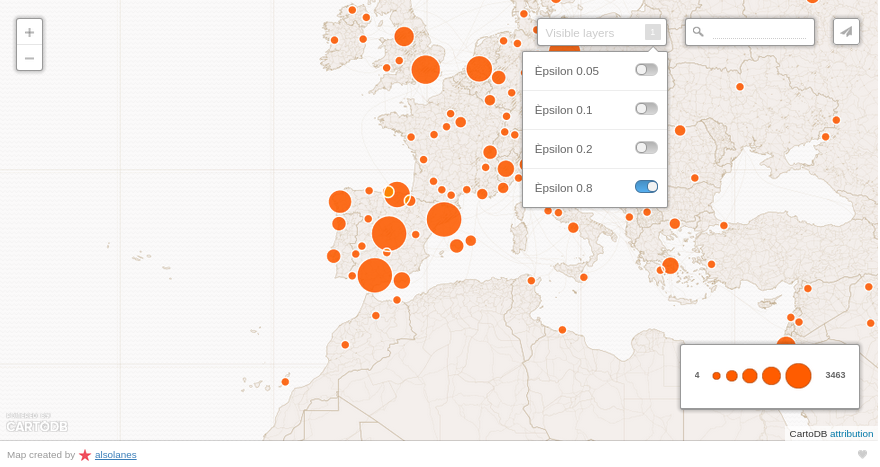
\includegraphics[width=12cm]{cartodb-res-4.png}
\caption{Mapa disponible per a la divulgació. Es mostren els resultats d'aplicar l'algorisme DBScan.}
\end{figure}
\newpage
\subsection{Divulgació dels resultats}
Per a permetre a tot el públic que ho desitgi accedir als resultats del projecte, també s'ha realitzat una pàgina web, sota el domini de github.io amb el procés explicat breument, on també s'hi adjunta el link al github del projecte, per si algun desenvolupador desitja analitzar o continuar el projecte.\\
La pàgina web del projecte és:
\begin{quote}
\centering
\textbf{\textit{alsolanes.github.io/TFG}}
\end{quote}

\begin{figure}[!htbp]
\centering
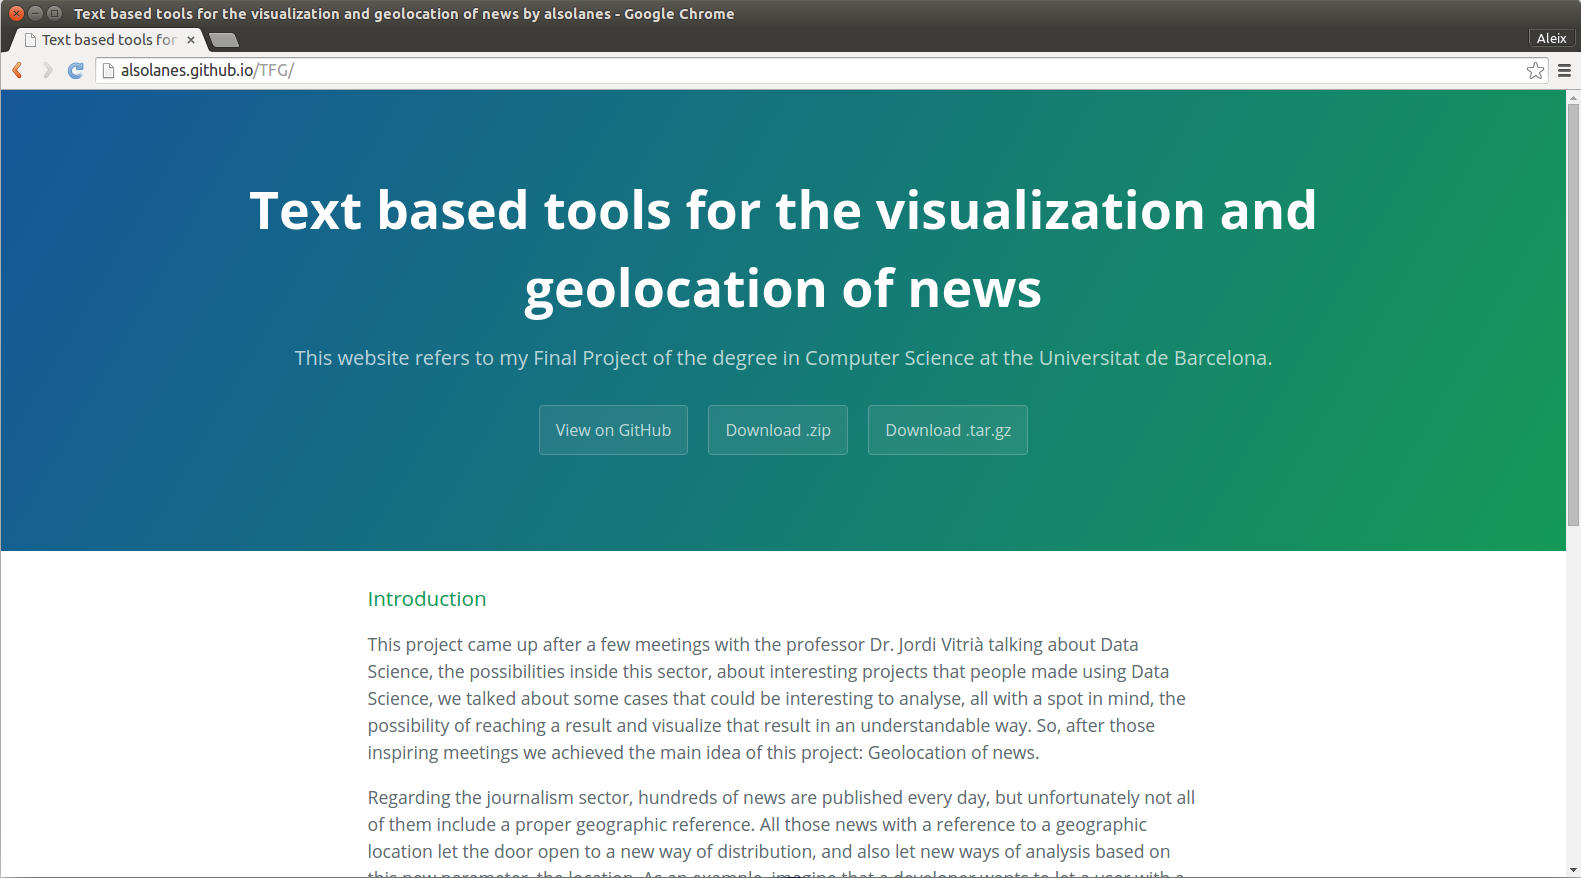
\includegraphics[width=12cm]{githubio.png}
\caption{Pàgina web del projecte.}
\end{figure}

\subsection{Passos extra per a l'execució de la pràctica}
En aquesta secció s'han explicat tots els passos per arribar al resultat final. Junt amb aquesta memòria, es disposa del codi del projecte en l'arxiu "\emph{TFG - Aleix Solanes.ipynb}". També es facilita una carpeta anomenada "Bases de dades" que inclou els següents fitxers, i que per a l'execució del projecte s'han de situar a la mateixa arrel que el fitxer iPython:
\begin{itemize}
\item antropònims.txt: conté una llista de noms de persona catalans.
\item CartoCat.xlsx: conté la informació relativa a les poblacions catalanes.
\item cities15000.txt: conté la informació de totes les poblacions a nivell mundial.
\item common\_names.txt: conté els noms de persona amb anglès i espanyol.
\item countryInfo.txt: conté informació de cada país.
\item iso-languagecodes.txt: conté informació dels codis ISO dels idiomes per exemple.
\end{itemize}
També s'adjunta la carpeta \emph{Resultats} amb els fitxers .csv que contenen els resultats de les ciutats trobades utilitzant clustering i sense, els quals són els que s'han pujat a la web CartoDB per a la seva visualització.\\
Una altra carpeta que es troba disponible és \emph{Obtenció de notícies}, la qual conté el programa python que s'ha utilitzat per automatitzar el procés d'obtenció de notícies.\\
A més s'adjunta la carpeta \emph{dump}, que conté les bases de dades de notícies i de ciutats utilitzades.\\
Per a la seva execució s'ha de fer un \emph{backup} de les dades en el sistema MongoDB instalat. Per a fer-ho s'ha d'executar el següent codi per a la base de notícies i de ciutats separadament (en cas de ser linux):

\emph{\$ mongorestore --db nom\_database path\_al\_fitxer\_bson}
\\\\
Per a l'execució del projecte també es necessita un fitxer anomenat \emph{alternateNames.txt}, però degut a la seva mida se n'adjunta el link de
descàrrega:\\\\
Enllaç personal:\\\\ \emph{https://mega.nz/\#!HlwEiJ6R!CFrNG2m3NOkJwJ2lC3yis1CQljQ8V\_C\_rbmkmuNT2nk}\\\\
Enllaç original:\\\\ \emph{http://download.geonames.org/export/dump/alternateNames.zip} (s'haurà de descomprimir primer)


\newpage


\section{Metodologia}
Organitzar el projecte correctament pot suposar la diferència entre l'èxit i el fracàs d'un projecte. Simplificar el desenvolupament i aprendre a distribuir-se bé el temps són dos dels objectius que es buscaven alhora de plantejar-se el desenvolupament del projecte.
És per això, que en veure la complexitat del projecte, es va decidir seguir uns principis bàsics principalment característics de les metodologies àgils.\\
Es mirava de minimitzar el risc d'error implementant durant tot el procés petites iteracions que permetien ampliar regularment la complexitat del codi, alhora que mirar de mantenir un codi estructurat, llegible i al mateix temps a cada iteració comprovar la veracitat dels resultats.\\
\subsection{Metodologia Àgil}
Són un conjunt de metodologies de desenvolupament que el que miren de potenciar és la possibilitat de realitzar canvis fins i tot en etapes avançades del projecte i minimitzar els errors que puguin aparèixer.\\
\subsubsection*{Desenvolupament iteratiu i incremental}
Es solen dividir les etapes d'un projecte en petites iteracions. Cada iteració, acaba amb el lliurament d'un projecte parcialment funcional, per tal d'anar veient els resultats a cada etapa i permetre visualitzar les seccions que necessiten millores o canvis des de bon principi. Aquestes iteracions solen tenir una durada d'entre una i quatre setmanes.\\
L'objectiu de tenir petits lliuraments és el de tenir al final de cada iteració, un software lliure d'errors, fiable i escalable, cosa que permet una evolució natural i adaptada per a futurs ampliacions i canvis.\\
\subsubsection*{Comunicació cara a cara amb el client al final de cada etapa}
En els desenvolupaments basats en equips, aquests solen ser pluridisciplinaris i participar en les diferents funcions d'un projecte: Planificació, Anàlisi de requisits, Disseny, Programació, Proves unitaries i Verificació de les proves. A més, en acabar cada iteració es sol mostrar el producte al client per a que pugui valorar el desenvolupament i aportar en el cas que ho consideri oportú la seva opinió. D'aquesta forma s'involucra més el client en el procés i així s'eviten disconformitats al final del projecte.\\
\subsubsection*{Repàs diari d'estat del projecte (daily meetings)}
Una característica habitual en les metodologies àgils, és una reunió diària que permet avaluar l'estat del projecte entre els diferents membres de l'equip. En aquestes reunions s'analitza el què es farà en aquell dia, i els impediments que bloquegen el projecte si n'hi ha.\\\\
Totes aquestes característiques es fonamenten en la qualitat del codi, aplicant automatismes per fer els tests unitaris, verificació de codi en parelles,...\cite{agile}\\\\
\subsubsection*{Scrum}
Un dels principals mètodes de desenvolupament amb metodologies àgils, és Scrum. El que pretén Scrum, és la creació d'equips autogestionats, autònoms, compromesos i pluridisciplinaris per tal d'assolir els objectius.\\
El projecte es divideix en iteracions anomenades "\emph{sprints}", que solen tenir una durada curta, d'entre una i quatre setmanes. Al final d'aquestes etapes es mostra el producte al client per a que pugui mostrar la seva opinió sobre aquest.\\
Cada iteració té unes fases marcades de planificació, anàlisi, codificació i proves unitàries sobre el codi desenvolupat.\\
Per a organitzar l'\emph{sprint}, primer es divideix el projecte en tasques atòmiques, per tal de millorar l'organització i facilitar la comprovació del funcionament de cada tasca. Cada tasca ha d'aportar valor per si sola, és a dir que ha de tenir una utilitat i una forma de verificar-la.\\\\
Es defineixen uns rols:
\begin{itemize}
\item Scrum Master: És la persona encarregada d'assegurar que els membres de l'equip segueixin la metodologia Scrum, i es compleixin tant a nivell organitzatiu dins l'equip com envers l'organització.
\item Product Owner: Representa als interessats en el projecte, és a dir, al client. Procura que el resultat del projecte sigui l'adequat.
\item Development team: L'equip encarregat de desenvolupar el projecte. Es recomanen equips petits d'entre tres i nou persones capaces de realitzar les diferents funcions en el projecte (ànalisi, disseny, desenvolupament, testeig, documentació).
\end{itemize}
Tal com s'ha definit scrum, no obstant no obstant, no és possible aplicar-ho al nostre projecte, per tant a continuació es descriuran les adaptacions necessàries per a la seva implementació en el projecte\cite{scrum}.
\subsection{Scrum aplicat al projecte}
El projecte tal com s'ha mencionat anteriorment ha procurat seguir els principis àgils, però adaptats donat que no hi havia un equip de treball, sinó que era un desenvolupament individual. Més concretament s'ha mirat d'adaptar les característiques de Scrum a un desenvolupament individual.\\
Algunes característiques d'Scrum, en mirar d'adaptar-lo al projecte s'han hagut de modificar o suprimir. Les característiques modificades respecte Scrum són les següents:
\begin{itemize}
\item Reunions: Es realitzaven les tasques de Sprint planning i anàlisi de l'anterior sprint en la mateixa reunió al final de cada sprint.
\item Supressió dels daily meetings.
\item Tutor com a Product Owner.
\end{itemize}
El projecte s'ha estructurat amb \emph{sprints} d'unes tres setmanes. En acabar cada iteració, ens reuníem amb el Dr. Jordi Vitrià, el tutor del projecte, per tal d'analitzar el desenvolupament realitzat en l'etapa acabada i planificar els objectius del següent sprint.\\
Acte seguit es realitzava un anàlisi dels requisits, i es començava el disseny de la etapa. Es mantenia un product backlog escrit en alt nivell, amb les descripcions genèriques dels requeriments i les funcionalitats que es desitjaven implementar, així com on es mantenien també errors a arreglar o modificacions.\\
En aquest moment es coneixia el què i el com fer l'etapa, i a partir d'aquí es començava el procés d'implementació.\\
Durant el procés d'implementació es mirava de potenciar la netedat en el codi per tal de poder ser capaç d'aplicar les millores o canvis que poguéssin sortir en un futur. També es procurava documentar mínimament el codi, mirant de no sobreexplicar funcionalitats per a facilitar-ne la comprensió.\\

\subsubsection*{Primera etapa: preparar les bases de dades de punts geogràfics}
La primera etapa del projecte es va destinar a investigar i experimentar amb diferents bases de dades fins a trobar-ne una de viable. Es van definir durant l'Sprint planning diferents projectes que s'havien de consultar per veure com enfocar el projecte. En el sprint backlog les tasques estaven centrades en la cerca i investigació de metodologies per a aconseguir la base de dades desitjada. Es va allargar en el temps més del previst ja que es va experimentar amb tres projectes diferents (SPARQL, DBPedia i finalment geonames.org) abans de trobar la base de dades final.\\
Es feien les proves unitàries per a comprovar si la base de dades complia els requeriments, fent consultes a aquesta base de dades amb una sèrie de ciutats preparades anteriorment, les quals contenien diferents característiques que feien que fos més probable que no es trobessin en una base de dades feble. Aquestes característiques podien ser el fet de tenir un nom complex, que fos una ciutat petita i poc coneguda, o que senzillament en anàlisis anteriors s'hagués trobat que en alguna altra base de dades no apareixia.\\
\subsubsection*{Segona etapa: algorisme bàsic per a localitzar ciutats}
En la primera part d'aquesta etapa, l'sprint backlog tenia entrades generals com ara: "identificar les paraules que començaven en majúscula i comprovar si són ciutats". No hi havia cap optimització, senzillament  es buscava un resultat en poc temps, per tant es comprovava si cada una d'aquestes paraules estava a la base de dades.\\ 
Per a començar es va fer un algorisme bàsic per tal d'aplicar la localització de ciutats en la base de dades de notícies.\\
En aquest moment es tenia una implementació funcional, però amb falsos positius i errades en algunes paraules que eren identificades erròniament.\\\\
\subsubsection*{Tercera etapa: visualització de les dades}
En aquesta etapa d'una durada d'un sprint es va investigar diferents formes de visualitzar les dades. Els elements presents en l'sprint backlog es centraven en visualitzar i comprovar la correcta visualització de les dades.\\
La visualització de les dades es va anar millorant durant diferents sprints, però en aquest primer, es va fer una primera aproximació.\\
\subsubsection*{Desenvolupament iteratiu}
Per a començar el desenvolupament iteratiu s'havia de disposar ja d'una base de notícies, per tant es va dur a terme la preparació d'aquesta base, per a poder anar-ne comprovant la fiabilitat.\\
Un cop arribat al final d'aquest procés, ja es tenia la base on anar ampliant i millorant funcionalitats. Es marcaven objectius en l'Sprint planning amb el tutor. A continuació es separava cada desenvolupament en tasques atòmiques que s'anotaven en l'sprint backlog.\\\\
Per anar seguint el desenvolupament, s'anava mantenint tot el codi en un repositori que permetia anar actualitzant per a preservar-lo i comprovar les diferents etapes per si en algun moment es desitjava retornar a una etapa anterior. Aquest, era un repositori git, gestionat sobre la base de github.com.\\
Cada etapa del procés anava incrementant la complexitat del projecte, i junt amb el projecte, la complexitat del codi. És per això, que s'ha anat documentant el codi per a facilitar la comprensió d'aquest en futures etapes, així com per a futurs possibles desenvolupadors que desitgin millorar o ampliar el codi.\\\\
Al finalitzar cada etapa, s'havia de comprovar la veracitat de les dades obtingudes, és per això que per a cada una de les tres etapes que tenia una iteració es realitzaven les proves següents:
\begin{itemize}
\item \textbf{Obtenir les bases de dades:} En les primeres iteracions les bases de dades anaven millorant, ja que s'anaven detectant errors. Per a comprovar cada una de les bases de dades es feien servir les següents tècniques:
\begin{itemize}
\item \textbf{Base de dades de Catalunya:} De forma experimental, s'anaven descobrint errors de poblacions que no es detectaven, i en aquest cas la solució era modificar la base de dades per a corregir l'error si era comú de varies poblacions(com ara no considerar els articles que es trobaven darrere d'una coma en el nom. exemple: Seu d'Urgell, la). Per a trobar aquests errors es comprovaven els resultats que es trobaven de les notícies, i es comprovaven amb la base de dades de localitats catalanes.
\item \textbf{Base de dades de la resta del món:} Es seguia el mateix procediment que amb la base de dades catalana, els errors es trobaven a base d'anar analitzant manualment els resultats obtinguts, al comparar-los amb els resultats esperats.
\item\textbf{ Base de dades de notícies:} Els errors trobats, majoritariament corresponien a errors de formatació de les dades, i s'anaven localitzant en analitzar manualment les dades obtingudes, o sinó durant el procés de testeig de tot el procés contra una base de dades de proves.
\end{itemize}
\item \textbf{Identificar localitats en un text}: Per anar analitzant les poblacions que no es reconeixien, es mantenien uns textos de prova on s'hi anava incloent les localitats que s'anava veient que donaven errors, o altres ciutats que donaven falsos positius. Per exemple el cas dels cognoms o dels noms, ja que si un nom o cognom era igual que un nom de ciutat, en un principi me'ls identificava com a localitats. 
\item \textbf{Visualització de les dades}: En aquest punt, es podia comprovar si alguna de les etapes anteriors no era correcta, com ara si mostrava ciutats estranyes, si mostrava ciutats en coordenades que no els pertocava, o si la quantitat d'aparicions d'una ciutat resultava sospitosa.
\end{itemize}

El procés descrit, s'anava repetint a cada iteració (sprint), fins a la última etapa. Aquesta es va centrar en només una etapa, la visualització.
\subsubsection*{Darrera etapa: visualització de les dades}
En aquesta etapa d'una durada de dos sprints, s'anava experimentant amb les diferents possibilitats que dóna CartoDB. Els objectius marcats estaven enfocats a permetre les diferents visualitzacions que s'han acabat implementant.\\
Aquesta etapa es va alternar amb la realització de la memòria.\\\\
Per a concretar més la planificació utilitzada es compararà la planificació inicial amb la que realment es va acabar utilitzant junt amb les referències temporals de cada etapa.
\subsection{Planificació inicial}
En plantejar les diferents etapes del projecte es van definir uns períodes per a planificar el projecte. Es considerava en un principi el següent calendari:
\begin{itemize}
\item Anàlisi de requisits: Abans de començar el projecte s'ha d'analitzar què ha de tenir tot el software, i què es busca per tal de poder saber què fer i quins són els objectius. Aquesta etapa estava previst que durés una setmana, la primera del projecte (Tercera setmana de febrer).
\item Anàlisi de les tecnologies i programari a utilitzar: Per a poder escollir les eines a utilitzar s'havia de fer un anàlisi més a fons de l'etapa de requisits i desglossar-ho amb tasques per veure cada tasca amb quines tecnologies es podria realitzar. És una etapa d'investigació de les tecnologies disponibles per a poder realitzar cada tasca. Aquesta tasca estava prevista que durés una setmana (última setmana de febrer).
\item Investigació i integració de la base de dades de localitats a utilitzar: La importància d'una bona base de dades és crucial per a obtenir uns resultats el més fiables possibles. A aquesta tasca se li estava previst assignar dues setmanes(Dues primeres setmanes de març).
\item Preparació de la base de dades de notícies: En un principi es considerava amb contar amb una base de dades real, el que va fer que en la planificació s'optés per a considerar dues setmanes per a la seva adequació als formats necessaris i la integració en l'entorn de desenvolupament (dues últimes setmanes de març).
\item Primeres aproximacions a geolocalitzar textos: Es crearia un primer algorisme que fes servir les diferents tecnologies i bases de dades descrites anteriorment per a obtenir els primers resultats. Es considerava una durada de dues setmanes (dues primeres setmanes d'abril).
\item Perfeccionament de la geolocalització de textos: Millorar l'algorisme per a la detecció de localitats, i retornar correctament utilitzant les bases de dades anteriors les dades que ens siguin necessàries per a la seva posterior visualització. Aquesta etapa estava previst que durés dues setmanes (dues últimes setmanes d'abril).
\item Visualització de les dades: En aquest punt ja es considerava que l'algorisme estaria funcionant correctament, per tant es volien dedicar dues setmanes a experimentar amb les possibilitats de CartoDB i preparar-ne les visualitzacions finals (Dues primeres setmanes de maig).
\item Redacció de la memòria: Aquesta tasca és important, és per això que es va considerar que la redacció de la memòria ocuparia unes 4 setmanes(dues últimes de maig i dues primeres de juny).
\end{itemize}
No obstant, aquesta planificació no va acabar sent la real, ja que algunes etapes s'allargaven més, apareixien modificacions respecte les tecnologies plantejades en un principi,... I finalment la planificació es va veure afectada com s'explica a continuació.

\begin{figure}[!htbp]
\centering
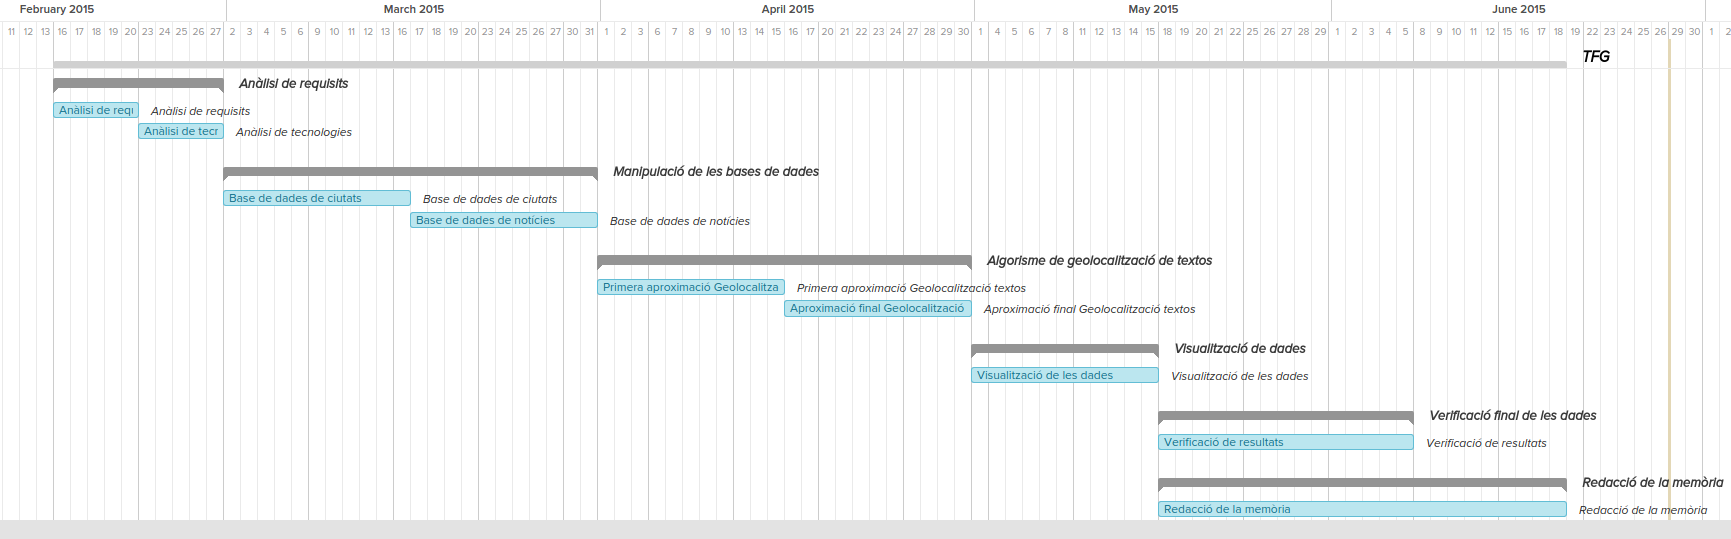
\includegraphics[width=16cm]{pla-inicial.png}
\caption{Diagrama de Gantt de la planificació inicial.}
\end{figure}
\subsection{Planificació real}
En plantejar les diferents etapes del projecte es van definir uns períodes per a planificar el projecte. Es considerava en un principi el següent calendari:
\begin{itemize}
\item Anàlisi de requisits: Aquesta etapa s'ha complert amb una setmana de duració.
\item Anàlisi de les tecnologies i programari a utilitzar: S'ha dut a terme amb una setmana de duració tal com estava previst. Si bé enmig de la realització del projecte s'han hagut de modificar algunes tecnologies per a millorar-ne resultats.
\item Investigació i integració de la base de dades de localitats a utilitzar: Aquest procés s'ha allargat més del previst, ja que s'ha hagut de subdividir en dos etapes diferenciades, obtenir una base de dades concreta per a les localitats de Catalunya, i una altra per a la localització de ciutats d'arreu del món. Finalment aquest procés ha acabat durant sis setmanes. No obstant s'han anat compaginant amb altres etapes.
\item Preparació de la base de dades de notícies: Aquesta etapa estava prevista que durés dues setmanes, i tot i que realment ha complert la duració prevista, s'ha hagut d'endarrerir en el temps per problemes amb la base de dades inicial. Finalment ha ocupat les tres darreres setmanes d'abril, i finalment les dades es comencen a obtenir correctament a finals d'abril-principis de maig.
\item Primeres aproximacions a geolocalitzar textos: Tal com estava previst, i per a complir els objectius temporals marcats, es va dur a terme aquesta tasca durant les dues primeres setmanes d'abril, complint el termini. Durant aquest període s'estava preparant al mateix temps la base de dades de ciutats. Per a comprovar els resultats es feien servir textos preparats expressament al no tenir la base de notícies acabada.
\item Perfeccionament de la geolocalització de textos: El perfeccionament de la geolocalització de notícies es va dur a terme durant les dues últimes setmanes d'abril, no obstant aquest procés es va allargar dues setmanes al comprovar l'algorisme amb la base de dades de notícies, ja que es trobaven nous casos susceptibles de ser analitzats.
\item Visualització de les dades: La visualització de dades es va començar a realitzar primer amb dades de prova, però en tenir la base de notícies es va començar a verificar sobre els resultats finals de la base de dades. Aquest procés es va allargar fins a la primera setmana de juny, ja que s'anava experimentant amb diferents tipus de visualització i s'anava adaptant als resultats obtinguts de la geolocalització.
\item Redacció de la memòria: En un principi es preveien unes quatre setmanes per a la redacció, no obstant el procés de desenvolupament es va allargar més del previst i va coincidir amb un increment de la càrrega de feina a la universitat (exàmens finals i entrega de pràctiques), el que va fer endarrerir l'inici de la redacció de la memòria. El procés finalment ha ocupat tres setmanes, si bé és cert que durant aquestes setmanes, la primera va ser destinada a la obtenció d'informació i creació de petits esbossos d'algunes parts de la memòria, i la redacció final es va dur a terme amb poc més de dues setmanes.
\end{itemize}

\begin{figure}[!htbp]
\centering
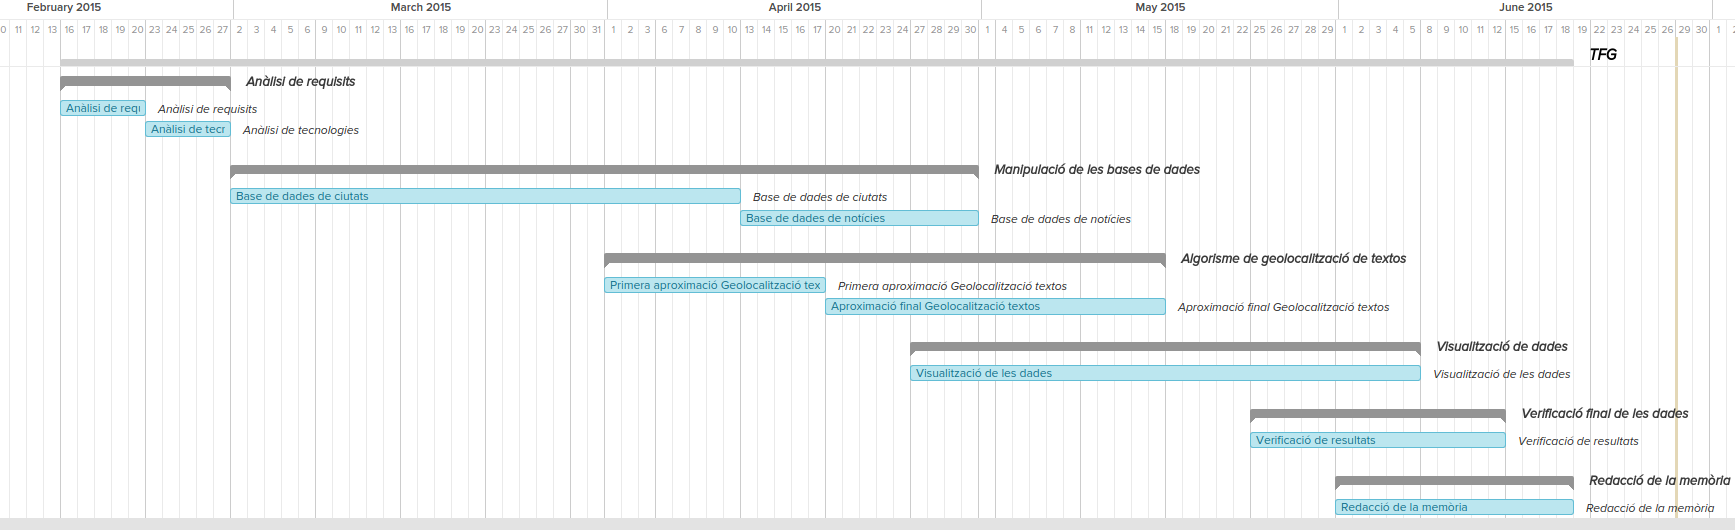
\includegraphics[width=16cm]{pla-final.png}
\caption{Diagrama de Gantt de la planificació final.}
\end{figure}

\newpage
\section{Resultats}
Per a avaluar la veracitat dels resultats, s'ha utilitzat una base de dades que conté notícies, junt amb la seva referència geogràfica. Aquesta base de dades, ha estat creada manualment, ja que no s'ha trobat cap base de referència que pogués facilitar el procés.\\

\begin{table}[!htbp]
\begin{center}
	\centering
    \begin{tabular}{| l | l | l |}
    \hline
    \textbf{} & \textbf{Quantitat} & \textbf{Percentatge}\\ \hline
    \textbf{Total esperades} & 220 & 100\% \\ \hline
    \textbf{Total trobades} & 218 & 99\%\\ \hline
    \textbf{Trobades correctament} & 205 & 93\%\\ \hline
    \textbf{No trobades} & 2 & 1\%\\ \hline
    \textbf{Falsos positius} & 13 & 5,9\%\\ \hline
    \end{tabular}
\end{center}
\caption{Encerts de l'algorisme respecte una base de dades de proves amb 200 notícies geolocalitzades manualment.}
\end{table}

Respecte una base de dades de 200 notícies, on en total hi ha 220 localitats (hi ha notícies amb més d'una referència geogràfica, i alguna que no en té), veiem que l'algorisme n'ha identificat 218, dels quals 13 han estat falsos positius. Dues ciutats no s'han trobat. El percentatge d'encerts és d'un 93\% en aquesta base de dades de 200 notícies.\\
Si s'analitzen els errors de falsos positius, la majoria són noms que s'han mencionat sense el respectiu cognom, o al revés, cognoms sense el nom davant. Per a separar aquests casos la solució sense fer un anàlisi del context és complicat, i donada la baixa freqüència de les aparicions s'ha decidit no afegir aquests casos en una llista negra per no tapar els resultats correctes d'aquestes localitats.\\\\
És cert que podria ser que en les més de 4500 notícies que té la base de dades els percentatges variïn, ja que per a localitzar els errors s'han analitzat sobretot els resultats respecte les 200 notícies.\\\\
\newpage
Tot seguit s'analitzaran les ciutats més freqüents en les notícies, per a fer-ho s'analitzarà la freqüència d'aparició de cada ciutat.\\

\begin{table}[!htbp]
\begin{center}
	\centering
    \begin{tabular}{| l | l | l |}
    \hline
    \textbf{Posició} & \textbf{Localitat} & \textbf{Freqüencia} \\ \hline
    1 	&	Barcelona		 	& 826 \\ \hline
	2	&	Madrid 				& 298 \\ \hline
	3	&	Manresa 			& 148 \\ \hline
	4	&	Lleida				& 116 \\ \hline
	5	&	Girona				& 113 \\ \hline
	6	&	Tarragona			& 82 \\ \hline
	7	&	Berga				& 76 \\ \hline
	8	&	Badalona			& 73 \\ \hline
	9	&	Berlín				& 65 \\ \hline
	10	&	Sabadell			& 61 \\ \hline	
	11	&	París				& 58 \\ \hline
	12	&	Nova York			& 52 \\ \hline 
	13	&	Terrassa			& 48 \\ \hline
	14	&	Sevilla				& 43 \\ \hline
	15	&	Londres				& 42 \\ \hline
	16	&	Reus				& 42 \\ \hline
	17	&	Munic				& 38 \\ \hline
	18	&	Mataró				& 37 \\ \hline
	19	&	Vic					& 33 \\ \hline
	20	&	Roma				& 29 \\ \hline
    \end{tabular}
\end{center}
\caption{Principals ciutats per freqüència d'aparició sobre un total de 5225 referències.}
\end{table}

Tal com es pot veure, la ciutat amb més representacions és ciutat, al considerar les notícies d'una sèrie de diaris digitals catalans, amb un focus especial sobre el territori català, té sentit que la principal ciutat en quant a aparicions sigui Barcelona.\\
La segona posició correspon a la ciutat de Madrid, a molta distància de Barcelona, també és lògic ja que tant en la secció d'esports com en la secció de política espanyola apareix freqüentment.\\ A partir d'aquí una sèrie de ciutats catalanes, d'on podem destacar que Manresa és la tercera ciutat més mencionada, per sobre de capitals de província com Lleida, Girona o Tarragona.\\
La primera ciutat de fora de l'estat Espanyol correspon a Berlín, durant el període d'obtenció de dades hi va haver la final de la Champions League de futbol, i aquesta es celebrava a la ciutat de Berlín, fet que juntament amb el fet que ja de per sí és una de les ciutats amb més importància a Europa per qüestions de política econòmica li atorguen segurament aquesta quantitat de referències.\\\\
A continuació mirarem l'evolució temporal en quant a les referències que es fan de tres ciutats representatives: Barcelona, Madrid i Berlín.

\begin{figure}[!htbp]
\centering
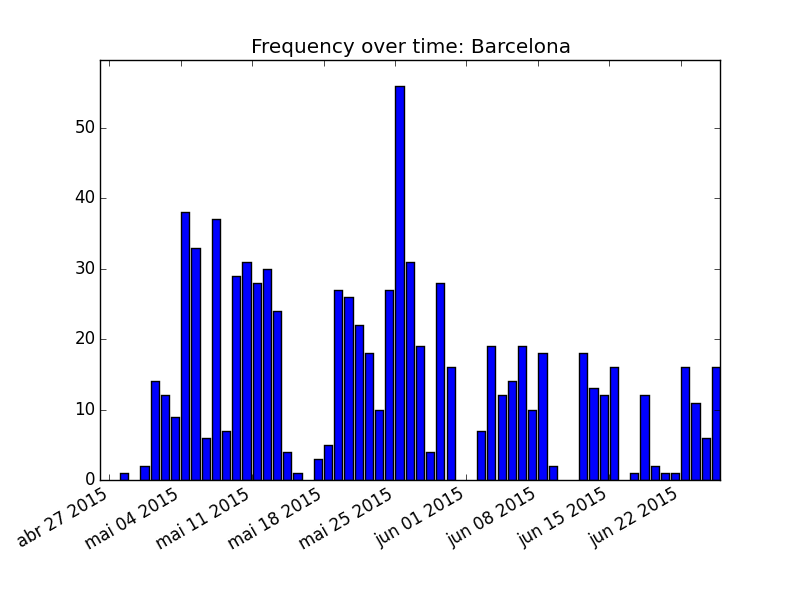
\includegraphics[width=10cm]{bcn-1.png}
\caption{Evolució temporal de les aparicions en les notícies de Barcelona.}
\end{figure}
En el gràfic podem veure un pic clar de referències de Barcelona. Aquest pic correspon al 25 de maig. Aquest dia es van registrar 56 referències de la ciutat de Barcelona en les notícies. Per comprendre el perquè, s'ha de tenir en compte que les eleccions municipals van tenir lloc el dia 24 de maig, i Barcelona va ser un focus d'atenció important, ja que hi havia un canvi de colors a l'ajuntament amb la presència d'un nou partit que irrompia amb molta força i es feia amb l'alcaldia de la ciutat.

\begin{figure}[!htbp]
\centering
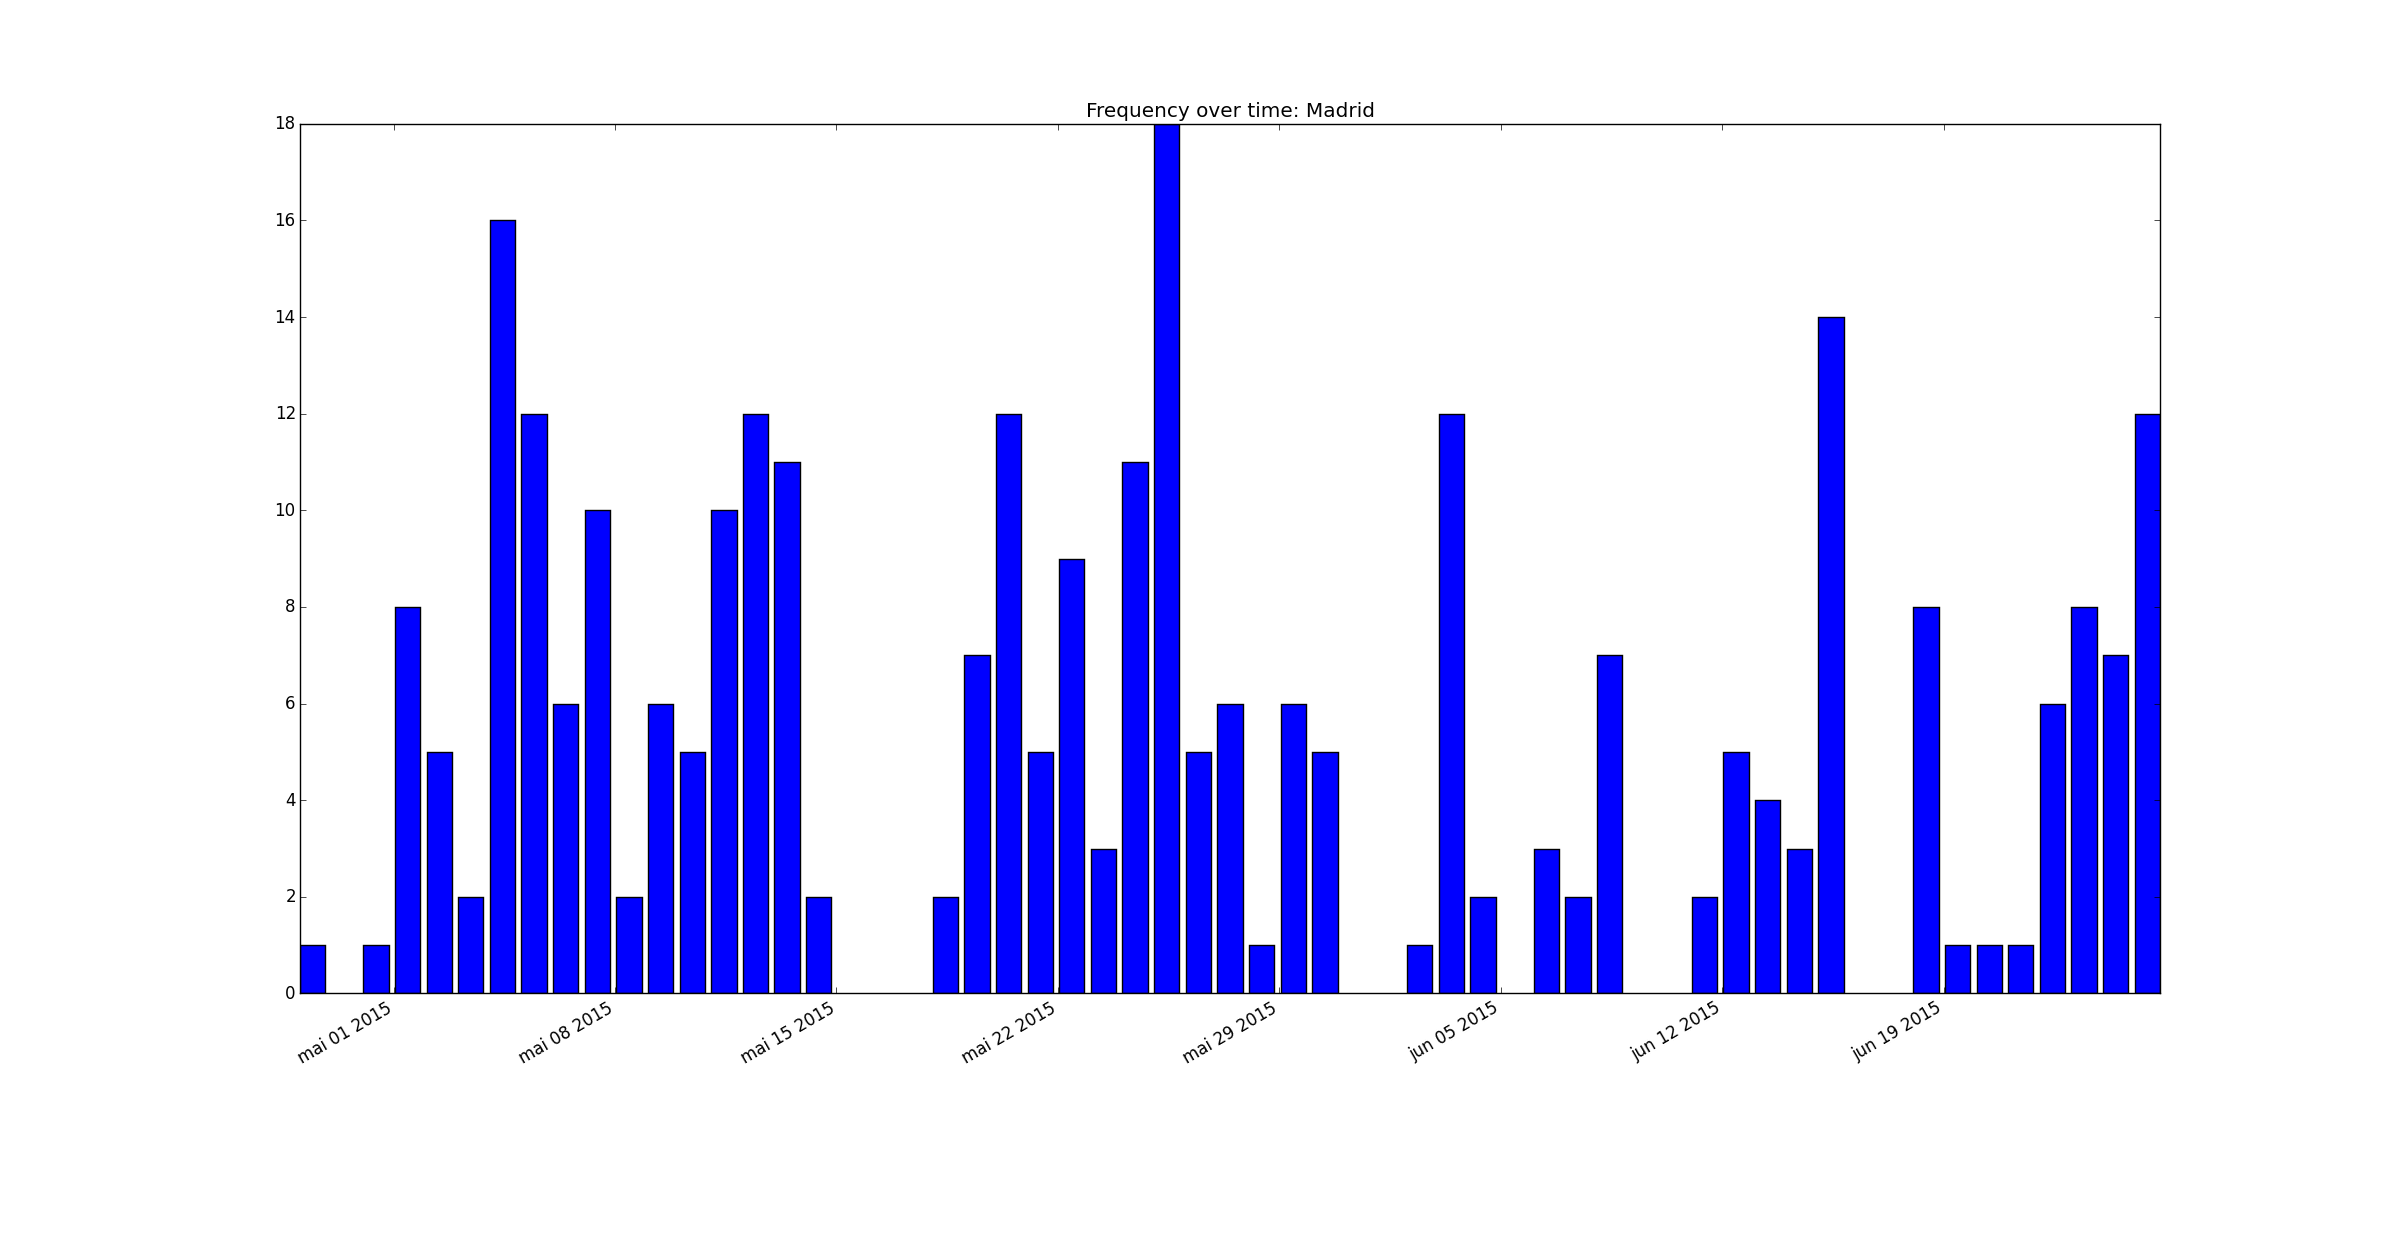
\includegraphics[width=13cm]{madrid-1.png}
\caption{Evolució temporal de les aparicions en les notícies de Madrid.}
\end{figure}
Igual que en l'anterior cas, la data on més es menciona la ciutat de Madrid correspon al 25 de maig, ja que a l'igual que a Barcelona un nou grup polític irrompia amb força a l'ajuntament i tenia opcions d'entrar a l'ajuntament. Finalment així va ser.\\
Observant les dades es veu un segon pic important que correspon al 4 de maig. Revisant el diari del dia en qüestió, es pot observar com el dia anterior s'havia publicat una enquesta sobre les eleccions municipals a Madrid, i a més coincidia amb les declaracions i anàlisi del partit que es jugaria l'endemà, el Reial Madrid - Juventus de Turí.\\
\begin{figure}[!htbp]
\centering
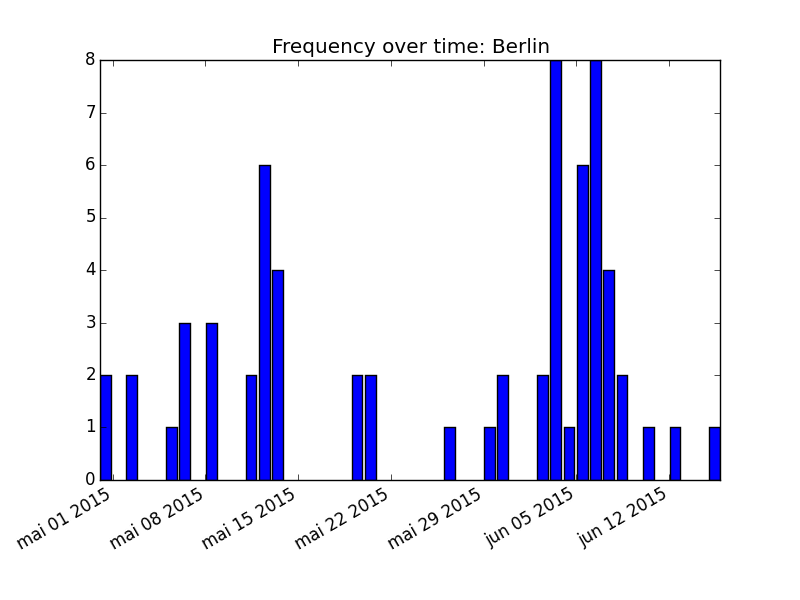
\includegraphics[width=10cm]{berlin-1.png}
\caption{Evolució temporal de les aparicions en les notícies de Berlín.}
\end{figure}

Finalment, analitzant el cas de Berlín, les seves aparicions tenen uns dies clau en què es publiquen més notícies de l'habitual sobre la ciutat. Són els dies al voltant del 6 de juny, data en què el Barça jugava la final de la Champions League a Berlín.\\\\
Per tant, després d'analitzar les dades, sembla que els pics més importants tenen una justificació de ser.\\\\
Respecte a les visualitzacions, s'ha de tenir present, que són la part més important per de cara a la divulgació del projecte, ja que de forma ràpida i senzilla es pot mostrar una gran quantitat d'informació, i alhora seria senzill deduir-ne errors si per exemple un simple punt aparegués enmig de l'aigua, o si la localitat més mencionada aparegués que fos un poble petit qualsevol.\\
En aquests mapes es poden veure de forma ràpida i senzilla l'abast de les notícies d'aquests diaris, i és especialment revelador mirar globalment el món i comprovar quines zones del món són les que es mencionen més. Es pot veure, com les ciutats que més es mencionen en els diaris utilitzats corresponen a les ciutats més importants a nivell econòmic o demogràfic. 

\begin{figure}[!htbp]
\centering
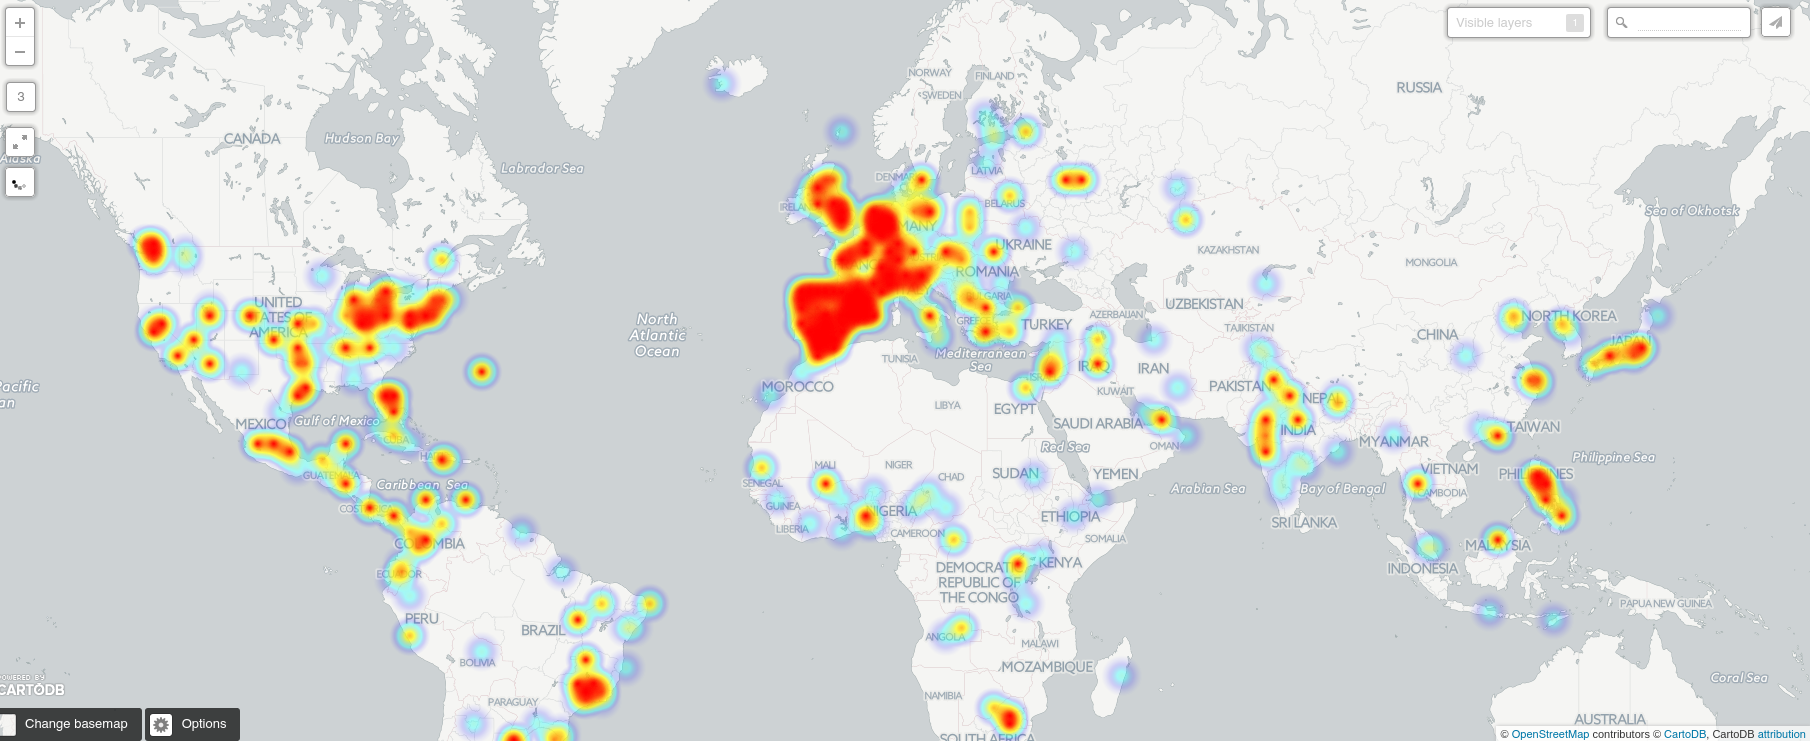
\includegraphics[width=12cm]{cartoDB-res-world.png}
\caption{Heat map global. Les localitats amb molt poques aparicions no es mostren.}
\end{figure}
\newpage
Per continents es pot comprovar com els principals continents dels quals es parla són Europa i Amèrica del Nord. També es pot comprovar com de tot el continent Asiàtic sobretot tenen presència les principals del sud del país com poden ser Hong Kong, Shanghai, Seül o Nova Delhi. Queden unes zones sense referències importants a les zones de l'interior i nord del continent asiàtic, l'interior de sud Amèrica, Oceania, la part més septentrional de nord Amèrica i gran part d'Àfrica. En molts casos es corresponen amb zones amb índexs de població baixos, fet que fa que o bé la base de dades no contingui informació sobre aquestes localitats o senzillament no apareguin perquè no es considerin importants per a publicar en els diaris catalans les notícies que puguin produir-se en aquestes zones.\\
\subsubsection*{Casos identificats que donen error}
Un dels casos més complicats d'analitzar són els casos en què una persona té com a nom o cognom, el nom d'una ciutat. En el cas que el nom estigui a la base de dades de noms i el cognom sigui una ciutat, aquest es gestiona, en cas contrari, pot donar un fals positiu.\\
Es poden produir errors amb casos com que el nom de la ciutat sigui un article en català (ciutat d'Un a la Índia, poble de Les a la Vall d'Aran, confusions en casos en què es parla d'un estat amb el mateix nom que la ciutat,...).\\
També hi haurà errors sempre que l'escriptor de la notícia no escrigui correctament el nom de la ciutat, amb majúscules i minúscules. S'ha intentat arreglar amb l'ús d'un corrector, però tot i arreglar els casos de petits errors, acabava donant problemes i donant falsos positius.\\\\
Respecte a l'obtenció de les notícies, s'han identificat alguns errors respecte a la data de publicació d'algunes notícies, que pel motiu que sigui no era la correcta en el moment de l'obtenció. Per a la visualització temporal, aquestes dades s'han filtrat, per evitar una visualització amb dades esbiaixades. La quantitat de dades incorrectes no arriba a les 15, pel que no és un error significatiu per a la visualització.

\subsubsection*{Limitacions}
La principal limitació que es pot trobar en el projecte, és en la identificació de les paraules susceptibles de ser una localitat. Una aproximació utilitzant aprenentatge automàtic, o aplicant tècniques d'anàlisi de llenguatge natural, podrien donar uns resultats més fiables, destriant casos que ara es donen com a resultats i que per context es pot veure que no és el resultat correcte.\\\\
El fet de tenir un punt dèbil en la identificació de ciutats ve marcada també pel fet que es depèn de que el periodista hagi escrit correctament el nom de la ciutat, i a més l'hagi escrit complet, ja que sovint s'abrevia el nom, com per exemple parlar de l'Hospitalet enlloc de l'Hospitalet de Llobregat.\\\\
Els diferents diaris digitals utilitzats fan servir un sistema RSS amb limitacions respecte el nombre de paraules que es comparteixen per aquesta tecnologia, per tant una de les millores més òbvies i urgents seria poder contar amb alguna font de dades amb la notícia completa.\\
També es considera una limitació important el fet de que les bases de dades no mantinguin una formatació idèntica per a cada paraula. Per exemple, en alguns casos podien contenir l'article davant del nom, i altres al final després d'una coma (i.e.: l'Hospitalet de Llobregat vs. Hospitalet de Llobregat, l').\\\\
Una altra limitació important, és en les possibilitats de visualització que pot donar CartoDB. Tot i que dóna moltes possibilitats, i una facilitat d'ús important, sempre s'està lligat a les funcions facilitades pel producte.\\
Una vegada un projecte es lliura de cara al públic, aquest pot rebre de forma contínua peticions de millora, notificacions d'errors,... Fins al moment, la identificació dels errors ha estat de forma manual, i considerant que en termes de llenguatge poden sorgir molts errors concrets i diferents els uns dels altres, són difícils de tractar per separat sense que una millora no afecti a altres resultats.

\newpage

\section{Conclusions i vies de continuació}
\subsection{Conclusions}
\subsubsection*{Conclusions referents a resultats}
Al iniciar el projecte, s'havien marcat cinc objectius ben diferenciats, i si un d'aquests objectius coixejava, la resta del projecte se'n veuria reflectida.\\
Una vegada s'ha acabat el projecte, es pot observar com en gran mesura s'han acomplert els objectius. A continuació s'analitzarà cada objectiu per separat:
\begin{enumerate}
\item \emph{Recopilar una sèrie de notícies per a ser analitzades}: S'ha aconseguit tenir una base de dades fiable i que es va ampliant automàticament dia a dia.
\item \emph{Crear una base de dades fiable amb les localitats que es tindran en compte per a la geolocalització de les notícies}: S'ha aconseguit una base de dades molt fiable per a la zona de Catalunya proporcionada per l'Institut Cartogràfic de Catalunya, i per a la resta del món s'ha aconseguit una base de dades que està sent actualitzada per la comunitat, però que per les dades del projecte han funcionat correctament.
\item \emph{Permetre identificar, donat un text, les paraules que són susceptibles de ser una localitat}: En els resultats respecte una base de dades de 200 notícies per a comprovar quantitativament l'encert, s'ha assolit un 93\% d'encerts. S'ha de tenir en compte que els errors s'han anat depurant respecte aquesta base de dades, pel que fora d'aquesta base de dades de test els percentatges podrien variar. No obstant, sense utilitzar tècniques d'anàlisi de context, ni aprenentatge automàtic, els resultats són satisfactoris considerant que no s'esperava la perfecció, sinó obtenir una mostra estadística que pogués mostrar la tendència general.
\item \emph{Fent servir les bases de dades anteriors, mostrar en un mapa els diferents punts trobats, per a mostrar tant l'evolució temporal, com el nombre total d'aparicions d'una localitat en les notícies}: La visualització de dades s'ha realitzat correctament en termes generals.
\item \emph{Crear una pàgina web per a mostrar-ne els resultats, així com a permetre que altres usuaris puguin continuar o analitzar-ne el desenvolupament}: La pàgina web ha estat realitzada sota el domini de github.io. L'objectiu s'ha pogut complir.
\end{enumerate}

Per tant, veient els resultats, es pot concloure que s'ha assolit l'objectiu general marcat en un principi.\\
\subsubsection*{Conclusions a nivell personal}
Ha resultat molt enriquidor i interessant anar veient com durant les diferents etapes sorgien diferents dificultats, i com en gran mesura s'han pogut superar totes. S'han vist tecnologies noves que fins al moment a nivell personal desconeixia (MongoDB, SPARQL, moltes llibreries noves, github.io,...), i el fet d'anar-les enllaçant entre elles fins a poder formar aquest projecte ha estat una feina dura però molt interessant.\\
S'ha pogut experimentar amb implementacions alternatives al llarg d'aquest projecte, i de fet han acabat classificant-se com a alternatives gràcies a haver trobat alguna implementació més efectiva, però el fet d'haver pogut explorar altres formes d'encarar el problema, ha fet que pogués arribar a tenir una visió més àmplia del projecte.\\
Si he de destacar algun punt important del projecte, destacaria el fet que m'ha permès veure que qualsevol obstacle que es pugui anar trobant, té solució, i que en molts casos més d'una. I la satisfacció no és només que els problemes tinguin solució, sinó que personalment els hagi pogut superar.\\\\
Aquest projecte, l'he pogut dur a terme gràcies al suport i la tutela del Dr. Jordi Vitrià, i que en les múltiples reunions que hem tingut al llarg del projecte m'ha anat introduint conceptes, anècdotes, o projectes curiosos al voltant de la temàtica que ens ocupava, i de Data Science en general. Això ha fet despertar més en mi les ganes de seguir aprenent en aquest camp.
\subsection{Vies continuació}
El projecte ha assolit els objectius marcats inicialment, però en tot moment s'ha hagut de ser conscient del temps del que es disposava. És per això que algunes de les idees que han anat apareixent al llarg del projecte s'han quedat com a punts de possibles millores.\\
El primer punt i més clar alhora de prosseguir amb el projecte, seria suprimir al màxim les limitacions esmentades anteriorment.\\
S'hauria de millorar la base de dades, actualment s'està limitat a que el nom de la ciutat escrita sigui idèntica a la que es troba a la base de dades. Es podrien afegir noms alternatius en aquesta base de dades, com per exemple termes com "la capital catalana" per a referir-se a Barcelona. \\
L'algorisme de detecció de localitats funciona força bé sempre i quant l'autor de la notícia n'escrigui els noms complets de les ciutats i de forma correcta. Per a solucionar aquesta limitació durant el projecte s'han contemplat dues opcions que podrien ajudar a millorar els resultats:
\begin{itemize}
\item Aplicació de tècniques d'aprenentatge automàtic que permetin geolocalitzar un text. Per exemple si dues localitats que tenen el mateix nom, una que està a la costa i l'altra a la muntanya, apareixen en un text, mitjançant les altres paraules del text es podria diferenciar quina de les dues localitats n'és la correcte. Ja que gràcies a un conjunt d'aprenentatge podríem saber quines paraules solen aparèixer al costat de cada localitat.
\item Mitjançant tècniques d'anàlisi de llenguatge natural, i més concretament utilitzant NER (named-entity recognition). Gràcies a aquestes tècniques podríem localitzar les diferents localitats, i mitjançant l'anàlisi del context, podríem saber si ens està parlat d'una localitat, d'un equip de futbol, d'un nom de persona...
\item Respecte a les limitacions amb CartoDB, es podria fer un desenvolupament, ja que CartoDB permet afegir extensions amb CSS i SQL. Aquesta implementació permetria per exemple mostrar finestres d'informació al clicar un punt de clusterització del mapa.
\end{itemize}

Unes altres vies de continuació, serien les de posar l'aplicació en nous escenaris. El primer cas que es veu en relacionar notícies amb punts geogràfics, seria el de desenvolupar una aplicació, que en funció de la posició geogràfica de l'usuari, li brindi unes notícies o unes altres.\\
Aquest punt, a més, permetria una millora automàtica de l'aplicació gràcies al feedback que podrien donar els usuaris. En el cas que els usuaris que estan a una ubicació ignorin una notícia sobre una localitat, es podria considerar que aquesta notícia o no està correctament geolocalitzada, o que senzillament no té interès a la zona, per tant tal com fa Google amb els resultats menys interessants, la notícia perdria importància i baixaria en el rànquing de notícies de la zona.\\\\
Una altra via de continuació seria mitjançant tècniques d'anàlisi del text, poder arribar a deduir si una notícia parla de forma positiva o negativa, o si és de temàtica esportiva, de successos,... D'aquesta forma es podrien arribar a conclusions de l'estil: a la ciutat X el 90\% de notícies que es publiquen són de caràcter negatiu. O que quan es parla de la ciutat Y sempre és pel seu equip de futbol.\\\\
De possibles continuacions n'hi hauria moltes, ja que les opcions són quasi infinites conforme s'afegeixen noves tecnologies i el problema esdevé més complexe. No obstant, les vies de continuació esmentades, són les que durant el projecte han aparegut com a idees de continuació, en definitiva són els passos que com a creador del projecte faria per a continuar millorant-ne la fiabilitat i les possibilitats.


\normalfont

\newpage

\begin{thebibliography}{50}
\bibitem{BigData} IBM Developer Networks: ¿Qué es Big Data?
\newline \texttt{https://www.ibm.com/developerworks/ssa/local/im/que-es-big-data/}

\bibitem{datascienceVenn} The Data Science Venn Diagram
\newline \texttt{http://drewconway.com/zia/2013/3/26/the-data-science-venn-diagram}

\bibitem{datasciencejob} Schutt, R.; O'Neil, C.: Doing Data Science: Straight Talk from the frontline, \textit{O'Reilly}, pàg. 1-15, 2014.

\bibitem{BOSS} Yahoo BOSS Geo Services: Overview
\newline \texttt{https://developer.yahoo.com/boss/geo/}

\bibitem{clavin} Repositori GITHUB del projecte CLAVIN
\newline \texttt{https://github.com/Berico-Technologies/CLAVIN}

\bibitem{textgrounder} Cohen, M.: TextGrounder: state of the art
\newline \texttt{https://mcohenlab.wordpress.com/textgrounder/}

\bibitem{googleAPI} The Google Geocoding API
\newline \texttt{https://developers.google.com/maps/documentation/geocoding/}

\bibitem{ara} Diari Ara: 1000 milions plens de dubtes [2/5/2015]
\newline \texttt{http://www.ara.cat/tema\_del\_dia/Segarra-Garrigues-milions-plens\\-dubtes\_0\_1349865056.html}

\bibitem{github} Github - About Github
\newline \texttt{https://github.com/about}

\bibitem{python} The Python Language
\newline \texttt{https://www.python.org/}

\bibitem{ipython} Jupiter and the future of Python
\newline \texttt{http://ipython.org/}

\bibitem{rss} The anatomy of an RSS feed
\newline \texttt{http://www.webreference.com/authoring/languages/xml/rss/feeds/index.html}

\bibitem{mongodb} MongoDB
\newline \texttt{https://www.mongodb.com/}

\bibitem{json} JSON - Introducing JSON
\newline \texttt{http://json.org}

\bibitem{cartodb} CartoDB - Maps for the web, made easy
\newline \texttt{http://cartodb.com}

\bibitem{geonames} Geonames - Gazeteer
\newline \texttt{http://download.geonames.org/export/dump/}

\bibitem{beautifulsoup} Beautiful Soup Documentation
\newline \texttt{https://beautiful-soup-4.readthedocs.org/en/latest/}

\bibitem{feedparser} Documentation - FeedParser
\newline \texttt{https://pythonhosted.org/feedparser/}

\bibitem{icc} Institut Cartogràfic i Geològic de Catalunya - Nomenclàtor
\newline \texttt{http://www.icc.cat/Home-ICC/Publicacions/Nomenclator}

\bibitem{github.io} How to use Github pages to make web sites while learning code
\newline \texttt{http://readwrite.com/2013/11/27/github-pages-explained}

\bibitem{nlp} Bird, S.; Klein, E.; Loper E.: Natural Language Processing with Python, \textit{O'Reilly}, pàg. preface, 1-33, 2013.

\bibitem{ner} Named Entity Definition
\newline \texttt{http://webknox.com/p/named-entity-definition}

\bibitem{sparql} Ducharme, B.: Learning SPARQL, \textit{O'Reilly}, pàg. 19-49, 2013.

\bibitem{dbpedia} DBPedia
\newline \texttt{http://dbpedia.org/}

\bibitem{time} Time - Time acess and conversions
\newline \texttt{https://docs.python.org/2/library/time.html}

\bibitem{softcatala} Corrector ortogràfic - SoftCatalà
\newline \texttt{https://www.softcatala.org/wiki/Projectes/Corrector\_ortografic}

\bibitem{nomsmon} Deron's Data Pages - Collections of interesting data, facts and wordlists.
\newline \texttt{http://deron.meranda.us/data/}

\bibitem{panda} The Data Science Lab - Beautiful plots with pandas and Matplotlib
\newline \texttt{https://datasciencelab.wordpress.com/2013/12/21/beautiful-plots\\-with-pandas-and-matplotlib/}

\bibitem{centroid} Mathwords: Centroid
\newline \texttt{http://www.mathwords.com/c/centroid.htm}

\bibitem{dbscan} Clustering to reduce Spatial Set Size - Geoff Boeing
\newline \texttt{http://geoffboeing.com/2014/08/clustering-to-reduce-spatial-data-set-size/}

\bibitem{agile} Agile Manifesto
\newline \texttt{http://agilemanifesto.org/}

\bibitem{scrum} Scrum Guides: The Scrum Guide
\newline \texttt{http://www.scrumguides.org/scrum-guide.html}



















\end{thebibliography}
\end{document} 

